%%%%%%%%%%%%%%%%%%%%%%%%%%%%%
% Standard header for working papers
%
% WPHeader.tex
%
%%%%%%%%%%%%%%%%%%%%%%%%%%%%%

\documentclass[11pt]{article}

%%%%%%%%%%%%%%%%%%%%
%% Include general header where common packages are defined
%%%%%%%%%%%%%%%%%%%%

% general packages without options
\usepackage{amsmath,amssymb,bbm}




%%%%%%%%%%%%%%%%%%%%
%% Idem general commands
%%%%%%%%%%%%%%%%%%%%
%% Commands

\newcommand{\noun}[1]{\textsc{#1}}


%% Math

% Operators
\DeclareMathOperator{\Cov}{Cov}
\DeclareMathOperator{\Var}{Var}
\DeclareMathOperator{\E}{\mathbb{E}}
\DeclareMathOperator{\Proba}{\mathbb{P}}

\newcommand{\Covb}[2]{\ensuremath{\Cov\!\left[#1,#2\right]}}
\newcommand{\Eb}[1]{\ensuremath{\E\!\left[#1\right]}}
\newcommand{\Pb}[1]{\ensuremath{\Proba\!\left[#1\right]}}
\newcommand{\Varb}[1]{\ensuremath{\Var\!\left[#1\right]}}

% norm
\newcommand{\norm}[1]{\| #1 \|}


% amsthm environments
\newtheorem{definition}{Definition}



%% graphics

% renew graphics command for relative path providment only ?
%\renewcommand{\includegraphics[]{}}








% geometry
\usepackage[margin=2cm]{geometry}

% layout : use fancyhdr package
\usepackage{fancyhdr}
\pagestyle{fancy}

\makeatletter

\renewcommand{\headrulewidth}{0.4pt}
\renewcommand{\footrulewidth}{0.4pt}
%\fancyhead[RO,RE]{\textit{Working Paper}}
\fancyhead[RO,RE]{\textit{ECTQG 2015}}
%\fancyhead[LO,LE]{G{\'e}ographie-Cit{\'e}s/LVMT}
\fancyhead[LO,LE]{An Algorithmic Systematic Review}
\fancyfoot[RO,RE] {\thepage}
\fancyfoot[LO,LE] {\noun{J. Raimbault}}
\fancyfoot[CO,CE] {}

\makeatother


%%%%%%%%%%%%%%%%%%%%%
%% Begin doc
%%%%%%%%%%%%%%%%%%%%%

\begin{document}







\title{\vspace{-2.5cm}Generation of Correlated Synthetic Data\\\medskip
\textit{Actes des Journées de Rochebrune 2016}
}
\author{\noun{Juste Raimbault}$^{1,2}$\\
$^{1}$ UMR CNRS 8504 Géographie-cités\\
$^{2}$ UMR-T IFSTTAR 9403 LVMT
}
\date{}%15 janvier 2016 - v1.01}


\maketitle

\justify

\vspace{-0.5cm}
\begin{abstract}
Generation of hybrid synthetic data resembling real data to some criteria is an important methodological and thematic issue in most disciplines which study complex systems. Interdependencies between constituting elements, materialized within respective relations, lead to the emergence of macroscopic patterns. Being able to control the dependance structure and level within a synthetic dataset is thus a source of knowledge on system mechanisms. We propose a methodology consisting in the generation of synthetic datasets on which correlation structure is controlled. The method is applied in a first example on financial time-series and allows to understand the role of interferences between components at different scales on performances of a predictive model. A second application on a geographical system is then proposed, in which the weak coupling between a population density model and a network morphogenesis model allows to simulate territorial configurations. The calibration on morphological objective on european data and intensive model exploration unveils a large spectrum of feasible correlations between morphological and network measures. We demonstrate therein the flexibility of our method and the variety of possible applications.
%La génération de données synthétiques hybrides similaires à des données réelles présente des enjeux méthodologiques et thématiques pour la plupart des disciplines dont l'objet est l'étude de systèmes complexes. Comme l'interdépendance entre les éléments constitutifs d'un système, matérialisée par leur relations, conduit à l'émergence de ses propriétés macroscopiques, une possibilité de contrôle de l'intensité des dépendances dans un jeu de données synthétiques est un instrument de connaissance du comportement du système. Nous proposons une méthodologie de génération de données synthétiques hybrides sur lequel la structure de correlation est contrôlée. La méthode est illustrée sur des séries temporelles financières et permet l'étude de l'interférence entre composantes à différentes fréquences sur la performance d'un modèle prédictif, en fonction des correlations entre composantes à différentes échelles. On présente ensuite une application à un système géographique, dans laquelle le couplage faible d'un modèle de distribution de densité de population avec un modèle de génération de réseau permet la simulation de configurations territoriales, qui sont calibrées selon des objectifs morphologiques sur l'ensemble de l'Europe. L'exploration intensive du modèle permet l'obtention d'un large spectre de valeurs pour la matrice de correlation entre mesures morphologiques et mesures du réseau. On démontre ainsi les possibilités d'applications variées et les potentialités de la méthode.
\end{abstract}

\medskip

\textbf{Keywords : } \textit{Synthetic Data ; Statistical Control ; Correlations ; Financial Time-series ; Land-use Transportation Interactions
}


%%%%%%%%%%%%%%%%%%%%%%
\section{Introduction}
%%%%%%%%%%%%%%%%%%%%%%

The use of synthetic data, in the sense of statistical populations generated randomly under constraints of patterns proximity to the studied system, is a widely used methodology, and more particularly in disciplines related to complex systems such as therapeutic evaluation~\cite{abadie2010synthetic}, territorial science~\cite{moeckel2003creating,pritchard2009advances}, machine learning~\cite{bolon2013review} or bio-informatics~\cite{van2006syntren}. It can consist in data desegregation by creation of a microscopic population with fixed macroscopic properties, or in the creation of new populations at the same scale than a given sample, with criteria of proximity to the real sample. These criteria will depend on expected applications and can for example vary from a restrictive statistical fit on given indicators, to weaker assumptions of similarity in aggregated patterns. In the case of chaotic systems, or systems where emergence plays a strong role, a microscopic property does not directly imply given macroscopic patterns, which reproduction is indeed one aim of modeling and simulation practices in complexity science. With the rise of new computational paradigms~\cite{arthur2015complexity}, data (simulated, measured or hybrid) shape our understanding of complex systems. Methodological tools for data-mining and modeling and simulation (including the generation of synthetic data) are therefore crucial to be developed.
%L'utilisation de données synthétiques, au sens de populations statistiques d'individus générées aléatoirement sous la contrainte de reproduire certaines caractéristiques du système étudié, est une pratique méthodologique largement répandue dans de nombreuses disciplines, et particulièrement pour des problématiques liées aux systèmes complexes, telles que par exemple l'évaluation thérapeutique~\cite{abadie2010synthetic}, l'étude des systèmes territoriaux~\cite{moeckel2003creating,pritchard2009advances}, l'apprentissage statistique~\cite{bolon2013review} ou la bio-informatique~\cite{van2006syntren}. Il peut s'agir d'une désagrégation par création d'une population au niveau microscopique présentant des caractéristiques macroscopiques données, ou bien de la création de nouvelles populations au même niveau d'agrégation qu'un échantillon donné avec un critère de ressemblance aux données réelles.  Le niveau de ce critère peut dépendra des applications attendues et peut par exemple aller de la fidélité des distributions statistiques pour un certain nombre d'indicateurs à des contraintes plus faibles de valeurs pour des indicateurs agrégés, c'est à dire l'existence de motifs macroscopiques similaires. Dans le cas de systèmes chaotiques ou présentant de fortes caractéristiques d'émergence, une contrainte microscopique n'implique pas nécessairement le respect des motifs macroscopiques, et arriver à les reproduire est justement un des enjeux des pratiques de modélisation et simulation en sciences de la complexité. La donnée, qu'elle soit simulée, mesurée ou hybride est au coeur de l'étude des systèmes complexes de par la maturation de nouvelles approches computationelles~\cite{arthur2015complexity}, il est donc essentiel d'étudier des procédures d'extraction d'information des données (fouille de données) et de simulation d'une information similaire (génération de données synthétiques).

Whereas first order (in the sense of distribution moments) is generally well used, it is not systematic nor simple to control generated data structure at second order, i.e. covariance structure between generated variables. Some specific examples can be found, such as in~\cite{ye2011investigation} where the sensitivity of discrete choices models to the distributions of inputs and to their dependance structure is examined. It is also possible to interpret complex networks generative models~\cite{newman2003structure} as the production of an interdependence structure for a system, contained within link topology. We introduce here a generic method taking into account dependance structure for the generation of synthetic datasets, more precisely with the mean of controlled correlation matrices.

%Si le premier ordre est de manière générale bien maîtrisé, il n'est pas systématique ni aisé de contrôler le second ordre, c'est à dire les structures de covariance entre les variables générées, même si des exemples spécifiques existent, comme dans~\cite{ye2011investigation} où la sensibilité des sorties de modèles de choix discrets à la forme des distributions des variables aléatoires ainsi qu'à leur structures de dépendance. Il est également possible d'interpréter les modèles de génération de réseaux complexes~\cite{newman2003structure} comme la création d'une structure d'interdépendance au sein d'un système, représentée par la topologie des liens. Nous proposons ici une méthode générique prenant en compte l'interdépendance lors de la génération de données synthétiques, sous la forme de correlations.

The rest of the paper is organized as follows. The generic method is formally described, to be then applied on very different examples both entering application frame. Each example can be read independently and illustrates potentialities of the method and possible technical limitations. We discuss then possible further developments and applications, in particular for a geographical system.
%La suite de l'article est organisée de la façon suivante. La méthode générique est décrite formellement, pour être appliquée sur deux exemples très différents mais rentrant dans ce même cadre. Chaque exemple peut être lu de manière indépendante et illustre les possibilités offertes par la méthode ainsi que des possibles obstacles à sa mise en oeuvre. Les implications et applications possibles sont ensuite discutées, notamment dans le cas de l'exemple d'un système géographique.


%%%%%%%%%%%%%%%%%%%%%%
\section{Method Formalization}
%%%%%%%%%%%%%%%%%%%%%%

Domain-specific methods aforementioned are too broad to be summarized into a same formalism. We propose a framework as generic as possible, centered on the control of correlations structure in synthetic data.
%L'ensemble des méthodologies mentionnées en introduction sont trop variées pour être résumées par un même formalisme. Nous proposons ici une formulation générique ne dépendant pas du domaine d'application, ciblée sur le contrôle de la structure de correlation des données synthétiques.

Let $\vec{X}_I$ a multidimensional stochastic process (that can be indexed e.g. with time in the case of time-series, but also space, or discrete set abstract indexation). We assume given a real dataset $\mathbf{X}=(X_{i,j})$, interpreted as a set of realizations of the stochastic process. We propose to generate a statistical population $\mathbf{\tilde{X}}=\tilde{X}_{i,j}$ such that
\begin{enumerate}
\item a given criteria of proximity to data is verified, i.e. given a precision $\varepsilon$ and an indicator $f$, we have $\norm{f(\mathbf{X})-f(\mathbf{\tilde{X}})} < \varepsilon$
\item level of correlation is controlled, i.e. given a matrix $R$ fixing correlation structure (symmetric matrix with coefficients in $[-1,1]$ and unity diagonal), we have $\hat{\Var{}}\left[(\tilde{X}_i)\right] = \Sigma R \Sigma$, where the standard deviation diagonal matrix $\Sigma$ is estimated on the synthetic population.
\end{enumerate}

%Soit un processus stochastique multidimensionnel $\vec{X}_I$ (l'ensemble d'indexation pouvant être par exemple le temps dans le cas de séries temporelles, l'espace, ou une indexation quelconque). On se propose, à partir d'un jeu de réalisations $\mathbf{X}=(X_{i,j})$, de générer une population statistique $\mathbf{\tilde{X}}=\tilde{X}_{i,j}$ telle que
%\begin{enumerate}
%\item d'une part un certain critère de proximité aux données est vérifié, i.e. étant donné une précision $\varepsilon$ et un indicateur $f$, $\norm{f(\mathbf{X})-f(\mathbf{\tilde{X}})} < \varepsilon$
%\item d'autre part le niveau de correlation est controlé, i.e. étant donné une matrice fixant une structure de covariance $R$, $\Varb{(\tilde{X}_i)} = R$, où la matrice de variance/covariance est estimée sur la population synthétique.
%\end{enumerate}

The second requirement will generally be conditional to parameter values determining generation procedure, either generation models being simple or complex ($R$ itself is a parameter). Formally, synthetic processes are parametric families $\tilde{X}_i[\vec{\alpha}]$. % TODO : explicit the fact that real data may come out of different parameter values ?
We propose to apply the methodology on very different examples, both typical of complex systems : financial high-frequency time-series and territorial systems. We illustrate the flexibility of the method, and claim to help building interdisciplinary bridges by methodology transposition and reasoning analogy. In the first case, proximity to data is the equality of signals at a fundamental frequency, to which higher frequency synthetic components with controlled correlations are superposed. It follows a logic of hybrid data for which hypothesis or model testing is done on a more realistic context than on purely synthetic data. In the second case, morphological calibration of a population density distribution model allows to respect real data proximity. Correlations of urban form with transportation network measures are empirically obtained by exploration of coupling with a network morphogenesis model. The control is in this case indirect as feasible space is empirically determined.
%La satisfaction du deuxième point sera généralement conditionnée par la valeur de paramètres, dont dépendra la procédure de génération, qu'il s'agisse de modèles simples ou complexes. Formellement, les processus synthétiques sont des familles paramétriques $\tilde{X}_i[\vec{\alpha}]$. Nous proposons de décliner cette méthode sur deux exemples très différents mais tous deux typiques des systèmes complexes : des séries temporelles financières à haute fréquence, et les systèmes territoriaux. On illustre ainsi la flexibilité de la logique, ouvrant des portes interdisciplinaires par l'exportation de méthodes ou raisonnements par exemple. Dans le premier cas, la proximité aux données est l'égalité des signaux à une fréquence fondamentale, auxquels on superpose des composantes synthétiques dont il est facile de contrôler le niveau de correlation. On se place dans une logique de données hybrides, pour tester des hypothèses ou modèles dans un contexte plus proche de la réalité que sur des données purement synthétiques. Dans le deuxième cas, la calibration morphologique d'un modèle de distribution de densité de peuplement permet de respecter le critère de proximité aux données. Les correlations de la forme urbaine avec celle d'un réseau de transport sont ensuite obtenues empiriquement par exploration du couplage avec un modèle de génération de réseau. Leur contrôle est dans ce cas indirect puisque constaté empiriquement.


%%%%%%%%%%%%%%%%%%%%%%
\section{Applications}
%%%%%%%%%%%%%%%%%%%%%%



%%%%%%%%%%%%%%%%%%%%%%
\subsection{Application : financial time-series}


%%%%%%%%%%%%%%%%%%%%%%
\subsubsection{Context}

Our first field of application is that of financial complex systems, of which captured signals, financial time-series, are heterogeneous, multi-scalar and highly non-stationary~\cite{mantegna2000introduction}. Correlations have already been the object of a broad bunch of related literature. For example, Random Matrix Theory allows to undress signal of noise, or at least to estimate the proportion of information undistinguishable from noise, for a correlation matrix computed for a large number of asset with low-frequency signals (daily returns mostly)~\cite{2009arXiv0910.1205B}. Similarly, Complex Network Analysis on networks constructed from correlations, by methods such as Minimal Spanning Tree~\cite{2001PhyA..299...16B} or more refined extensions developed for this purpose~\cite{tumminello2005tool}, yielded promising results such as the reconstruction of economic sectors structure. At high frequency, the precise estimation of of interdependence parameters in the framed of fixed assumptions on asset dynamics, has been extensively studied from a theoretical point of view aimed at refinement of models and estimators~\cite{barndorff2011multivariate}. Theoretical results must be tested on synthetic datasets as they ensure a control of most parameters in order to check that a predicted effect is indeed observable \emph{all things equal otherwise}. For example, \cite{potiron2015estimation} obtains a bias correction for the \emph{Hayashi-Yoshida} estimator (used to estimate integrated covariation between two brownian at high frequency in the case of asynchronous observation times) by deriving a central limit theorem for a general model that endogeneize observation times. Empirical confirmation of estimator improvement is obtained on a synthetic dataset at a fixed correlation level.

%Un premier domaine d'application proposé pour notre méthode est celui des séries temporelles financières, signaux typiques de systèmes complexes hétérogènes et multiscalaires~\cite{mantegna2000introduction} et pour lesquels les corrélations ont fait l'objet d'abondants travaux. Ainsi, l'application de la théorie des matrices aléatoires peut permettre de débruiter, ou du moins d'estimer la part de signal noyée dans le bruit, une matrice de correlations pour un grand nombre d'actifs échantillonnés à faible fréquence (retours journaliers par exemple)~\cite{2009arXiv0910.1205B}. De même, l'analyse de réseaux complexes construits à partir des corrélations, selon des méthodes type arbre couvrant minimal~\cite{2001PhyA..299...16B} ou des extensions raffinées pour cette application précise~\cite{tumminello2005tool}, ont permis d'obtenir des résultats prometteurs, tels la reconstruction de la structure économique des secteurs d'activités. A haute fréquence, l'estimation précise de paramètres d'interdépendance dans le cadre d'hypothèses fixées sur la dynamique, fait l'objet d'importants travaux théoriques dans un but de raffinement des modèles et des estimateurs~\cite{barndorff2011multivariate}. Les résultats théoriques doivent alors être testés sur des jeux de données synthétiques, qui permettent de contrôler un certain nombre de paramètres et de s'assurer qu'un effet prédit par la théorie est bien observable \emph{toutes choses égales par ailleurs}. Par exemple, \cite{potiron2015estimation} dérive une correction du biais de l'estimateur de \emph{Hayashi-Yoshida} qui est un estimateur de la covariance de deux browniens corrélés à haute fréquence dans le cas de temps d'observation asynchrones, par démonstration d'un théorème de la limite centrale pour un modèle généralisé endogénéisant les temps d'observations. La confirmation empirique de l'amélioration de l'estimateur est alors obtenue sur un jeu de données synthétiques à un niveau de corrélation fixé.


%%%%%%%%%%%%%%%%%%%%%%
\subsubsection{Formalization}

\paragraph{Framework}

We consider a network of assets $(X_i(t))_{1\leq i \leq N}$ sampled at high-frequency (typically 1s). We use a multi-scalar framework (used e.g. in wavelet analysis approaches~\cite{ramsey2002wavelets} or in multi-fractal signal processing~\cite{bouchaud2000apparent}) to interpret observed signals as the superposition of components at different time scales : $X_i=\sum_{\omega}{X_i^{\omega}}$. We denote by $T_i^{\omega} = \sum_{\omega' \leq \omega} X_i^{\omega}$ the filtered signal at a given frequency $\omega$. A recurrent problem in the study of complex systems is the prediction of a trend at a given scale. It can be viewed as the identification of regularities and their distinction from components considered as random\footnote{see~\cite{gell1995quark} for an extended discussion on the construction of \emph{schema} to study complex adaptive systems (by complex adaptive systems).}. For the sake of simplicity, we represent such a process as a trend prediction model at a given temporal scale $\omega_1$, formally an estimator $M_{\omega_1} : (T_i^{\omega_1}(t'))_{t'<t} \mapsto \hat{T_i}^{\omega_1}(t)$ which aims to minimize error on the real trend $\norm{T_i^{\omega_1} - \hat{T}_i^{\omega_1}}$. In the case of autoregressive multivariate estimators, the performance will depend among other parameters on respective correlations between assets. It is thus interesting to apply the method to the evaluation of performance as a function of correlation at different scales. We assume a Black-Scholes dynamic for assets~\cite{jarrow1999honor}, i.e. $dX = \sigma\cdot dW$, with $W$ Wiener process. Such a dynamic model allows an easy modulation of correlation levels.


\paragraph{Data generation}

We can straightforward generate $\tilde{X}_i$ such that $\Varb{\tilde{X}_i^{\omega_1}}=\Sigma R \Sigma$ (with $\Sigma$ estimated standard deviations and $R$ fixed correlation matrix) and verifying $X_i^{\omega \leq \omega_0} = \tilde{X}_i^{\omega \leq \omega_0}$ (data proximity indicator : components at a lower frequency than a fundamental frequency $\omega_0 < \omega_1$ are identical). We use therefore the simulation of Wiener processes with fixed correlation. Indeed, if $dW_1 \indep dW_1^{\indep}$ (and $\sigma_1 < \sigma_2$ indicatively, assets being interchangeable), then
\[
W_2 = \rho_{12}W_1 + \sqrt{1-\frac{\sigma_1^2}{\sigma_2^2}\cdot\rho_{12}^2}\cdot W_1^{\indep}
\]
is such that $\rho(dW_1,dW_2)=\rho_{12}$. Next signals are constructed the same way by Gram orthonormalization. We isolate the component at the desired frequency $\omega_1$ by filtering the signal, i.e. $\tilde{X}_i^{\omega_1} = W_i - \mathcal{F}_{\omega_0}[W_i]$ (with $\mathcal{F}_{\omega_0}$ low-pass filter with cut-off frequency $\omega_0$). We reconstruct then the hybrid synthetic signals by 
\begin{equation}
\tilde{X}_i = T_i^{\omega_0} + \tilde{X}_i^{\omega_1}
\end{equation}


\subsubsection{Implementation and Results}

\paragraph{Methodology}

The method is tested on an example with two assets from foreign exchange market (EUR/USD and EUR/GBP), in a six month period from June 2015 to November 2015. Data\footnote{obtained from \texttt{http://www.histdata.com/}, without specified licence. For the respect of copyright, only cleaned and filtered at $\omega_m$ data are made openly available.} cleaning, starting from original series sampled at a frequency around 1s, consists in a first step to the determination of the minimal common temporal range (missing sequences being ignored, by vertical translation of series, i.e. $S(t):=S(t)\cdot \frac{S(t_{n})}{S(t_{n-1})}$ when $t_{n-1},t_n$ are extremities of the ``hole'' and $S(t)$ value of the asset, what is equivalent to keep the constraint to have returns at similar temporal steps between assets). We study then \emph{log-prices} and \emph{log-returns}, defined by $X(t):=\log{\frac{S(t)}{S_0}}$ and $\Delta X (t) = X(t) - X(t-1)$. Raw data are filtered at a maximal frequency $\omega_m = 10\textrm{min}$ (which will be the maximal frequency for following treatments) for concerns of computational efficiency\footnote{as time-series are then sampled at $3\cdot\omega_m$ to avoid aliasing, a day of size 86400 for 1s sampling is reduced to a much smaller size of 432.}. We use a non-causal gaussian filter of total width $\omega$. We fix the fundamental frequency $\omega_0=24\textrm{h}$ and we propose to construct synthetic data at frequencies $\omega_1 = 30\textrm{min},1\textrm{h},2\textrm{h}$. See Fig.~\ref{fig:example_signal} for an example of signal structure at these different scales.

%La méthode est testée sur un exemple de deux actifs du marché des devises (EUR/USD et EUR/GBP), sur une période de 6 mois de juin 2015 à novembre 2015. Le nettoyage des données\footnote{obtenues depuis \texttt{http://www.histdata.com/}, sans licence spécifiée, les données nettoyées et filtrées à $\omega_m$ uniquement sont mises en accessibilité pour respect du copyright.}, originellement échantillonnées à l'ordre de la seconde, consiste dans un premier temps à la détermination du support temporel commun maximal (les séquences manquantes étant alors ignorées, par translation verticale des séries, i.e. $S(t):=S(t)\cdot \frac{S(t_{n})}{S(t_{n-1})}$ lorsque $t_{n-1},t_n$ sont les extrémités du ``trou'' et $S(t)$ la valeur de l'actif, ce qui revient à garder la contrainte d'avoir des retours à pas de temps similaires entre actifs).On étudie alors les \emph{log-prix} et \emph{log-retours}, définis par $X(t):=\log{\frac{S(t)}{S_0}}$ et $\Delta X (t) = X(t) - X(t-1)$. Les données brutes sont filtrées à une fréquence $\omega_m = 10\textrm{min}$ (qui sera la fréquence maximale d'étude) pour un souci de performance computationnelle. On utilise un filtre gaussien non causal de largeur totale $\omega$. On fixe $\omega_0=24\textrm{h}$ et on se propose de construire des données synthétiques aux fréquences $\omega_1 = 30\textrm{min},1\textrm{h},2\textrm{h}$. Voir la figure~\ref{fig:example_signal} pour un exemple de la structure du signal à ce différentes échelles.


%%%%%%%%%%%%%%%%%%%
\begin{figure}%[h!]
\centering
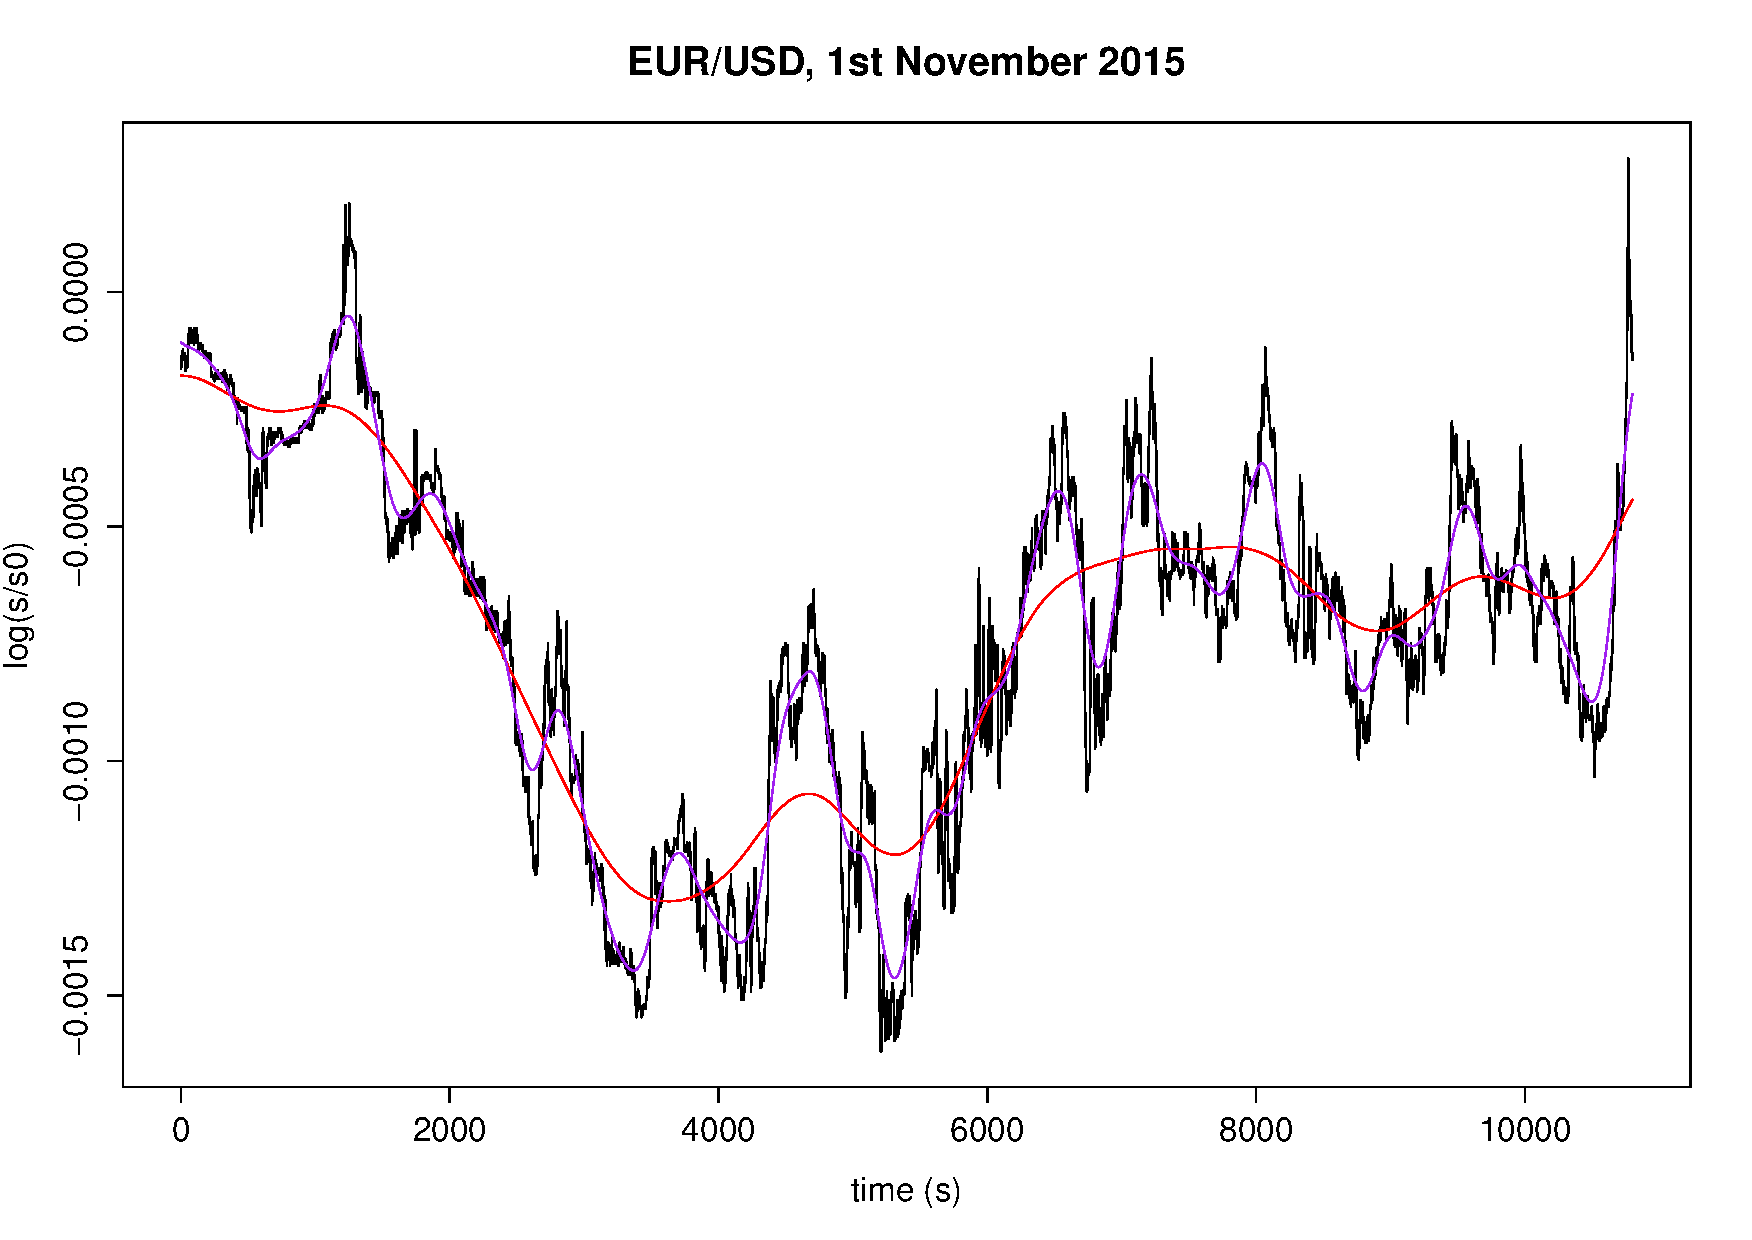
\includegraphics[width=0.6\textwidth,height=0.25\textheight]{figures/asset/ex_filtering}
\caption{\textbf{Example of the multi-scalar structure of the signal, basis of the construction of synthetic signals | } \emph{Log-prices} are represented on a time window of around 3h for November 1st 2015 for asset EUR/USD, with 10min (purple) and 30min trends.}
\label{fig:example_signal}
\end{figure}
%%%%%%%%%%%%%%%%%%%

% TODO : Q add examples of synthetic signal ?

It is crucial to consider the interference between $\omega_0$ and $\omega_1$ frequencies in the reconstructed signal : correlation indeed estimated is 
\[
\rho_{e} = \rho \left[ \Delta \tilde{X}_1 , \Delta \tilde{X}_2 \right] = \rho \left[ \Delta T_1^{\omega_0} + \Delta \tilde{X}_1^{\omega} , \Delta T_2^{\omega_0} + \Delta \tilde{X}_2^{\omega}\right]
\]
what yields in the reasonable limit $\sigma_1 \gg \sigma_0$ (fundamental frequency small enough), when $\Covb{\Delta \tilde{X}_i^{\omega_1}}{\Delta X_j^{\omega}}=0$ for all $i,j,\omega_1 > \omega$ and returns centered at any scale, the correction on effective correlation due to interferences : we have at first order the expression of effective correlation

\begin{equation}
\label{eq:eff_corr}
\rho_e = \left[ \varepsilon_1 \varepsilon_2 \rho_0 + \rho \right] \cdot \left[ 1 - \frac{1}{2}\left(\varepsilon_1^2 + \varepsilon_2^2 \right) \right]
\end{equation}

{\noindent}what gives the correlation that we can effectively simulate in synthetic data.

Correlation is estimated by Pearson method, with estimator for covariance corrected for bias, i.e.
\[
\hat{\rho}[X1,X2] = \frac{\hat{C}[X1,X2]}{\sqrt{\hat{\Var{}}[X1]\hat{\Var{}}[X2]}}\]
, where $\hat{C}[X1,X2] = \frac{1}{(T-1)}\sum_{t} X_1(t)X_2(t) - \frac{1}{T\cdot (T-1)} \sum_t X_1(t) \sum_t X_2(t)$ and $\hat{\Var{}}[X] = \frac{1}{T}\sum_t{X^2(t)}-\left(\frac{1}{T}\sum_tX(t)\right)^2$.


The tested predictive model $M_{\omega_1}$ is a simple \emph{ARMA} for which parameters $p=2,q=0$ are fixed (as we do not create lagged correlation, we do not expect large orders of auto-regression as these kind of processes have short memory for real data ; furthermore smoothing is not necessary as data are already filtered). It is however applied in an adaptive way\footnote{adaptation level staying low, as parameters $T_W,p,q$ and model type do not vary. We are positioned within the framework of~\cite{potiron2016estimating} which assumes a locally parametric dynamic but for which meta-parameters are fixed. We could imagine a variable $T_W$ which would adapt for the best local fit, the same way parameters are estimated in bayesian signal processing by augmentation of the state with parameters.}. More precisely, given a time window $T_W$, we estimate for any $t$ the model on $[t-T_W+1,t]$ in order to predict signals at $t+1$.

%Le modèle de prédiction $M_{\omega_1}$ testé est simplement un modèle \emph{ARMA} pour lequel on fixe les paramètres $p=2,q=0$ (on ne créée pas de correlation retardée, on ne s'attend donc pas à de grand ordre d'auto-regression, les signaux originaux étant à mémoire relativement courte ; de plus le lissage n'est pas nécessaire puisqu'on travaille sur des données filtrées), appliqué de manière adaptative\footnote{il s'agit d'un niveau d'adaptation relativement faible, les paramètres $T_W,p,q$ et même le type de modèle restant fixés. On se place ainsi dans le cadre de~\cite{potiron2016estimating} qui suppose une dynamique localement paramétrique, mais pour lequel on fixe les méta-paramètres de la dynamique. On pourrait imaginer estimer un $T_W$ variable qui s'adapterait pour une meilleure estimation locale, à l'image de l'estimation de paramètres en traitement du signal bayesien effectuée via augmentation de l'état par les paramètres.}. Plus précisément, étant donné une fenêtre temporelle $T_W$, on estime pour tout $t$ le modèle sur $[t-T_W+1,t]$ afin de prédire les signaux à $t+1$.


\paragraph{Implementation}

Experiments are implemented in \texttt{R} language, using in particular the \texttt{MTS}~\cite{Tsay:2015xy} library for time-series models. Cleaned data and source code are openly available on the \texttt{git} repository of the project\footnote{at \texttt{https://github.com/JusteRaimbault/SynthAsset}}. 

%L'implémentation est faite en language R, utilisant en particulier la bibliothèque \texttt{MTS}~\cite{Tsay:2015xy} pour les modèles de séries temporelles. Les données nettoyées et le code source sont disponibles de manière ouverte sur le dépôt \texttt{git} du projet\footnote{at \texttt{https://github.com/JusteRaimbault/SynthAsset}}.


\paragraph{Results}



Figure~\ref{fig:effective_corrs} gives effective correlations computed on synthetic data. For standard parameter values (for example $\omega_0=24\textrm{h}$, $\omega_1=2\textrm{h}$ and $\rho=-0.5$), we find $\rho_0\simeq 0.71$ et $\varepsilon_i \simeq 0.3$ what yields $\left| \rho_e - \rho \right|\simeq 0.05$. We observe a good agreement between observed $\rho_e$ and values predicted by~\ref{eq:eff_corr} in the interval $\rho \in [-0.5,0.5]$. On the contrary, for larger absolute values, a deviation increasing with $\left|\rho\right|$ and as $\omega_1$ decreases : it confirms the intuition that when frequency decreases and becomes closer to $\omega_0$, interferences between the two components are not negligible anymore and invalidate independence assumptions for example. 


%La figure~\ref{fig:effective_corrs} donne les correlations effectives calculées sur les données synthétiques. Pour des valeurs standard des paramètres (par exemple pour $\omega_0=24\textrm{h}$, $\omega_1=2\textrm{h}$ et $\rho=-0.5$), on a $\rho_0\simeq 0.71$ et $\varepsilon_i \simeq 0.3$ et ainsi $\left| \rho_e - \rho \right|\simeq 0.05$. On constate dans l'intervalle $\rho \in [-0.5,0.5]$ un bon accord entre la valeur $\rho_e$ prédite par~\ref{eq:eff_corr} et les valeurs observées, et une déviation pour de plus grandes valeurs absolues, d'autant plus grande que $\omega_1$ est petit : cela confirme l'intuition que lorsque la fréquence descend et se rapproche de $\omega_0$, les interférences entre les deux composantes vont devenir non négligeables et invalider les hypothèses d'indépendance par exemple.


We apply then the predictive model described above to synthetic data, in order to study its mean performance as a function of correlation between signals. Results for $\omega_1 = 1\textrm{h},1\textrm{h}30,2\textrm{h}$ are shown in Fig.~\ref{fig:model_perf}. The a priori counter-intuitive result of a maximal performance at vanishing correlation for one of the assets confirms the role of synthetic data to better understand system mechanisms : the study of lagged correlations shows an asymmetry in the real data that we can understand at a daily scale as an increased influence of EUR/GBP on EUR/USD with a rough two hours lag. The existence of this \emph{lag} allows a ``good'' prediction of EUR/USD thanks to fundamental component. This predictive power is perturbed by added noises in a way that increases with their correlation. The more noises correlated are, the more he model will take them into account and will make false predictions because of the markovian character of simulated brownian\footnote{the model used has theoretically no predictive power at all on pure brownian}.

%On applique ensuite le modèle prédictif décrit ci-dessus aux données synthétiques, afin d'étudier sa performance moyenne en fonction du niveau de correlation des données. Les résultats pour $\omega_1 = 1\textrm{h},1\textrm{h}30,2\textrm{h}$ sont présentés en figure~\ref{fig:model_perf}. Le résultat a priori contre-intuitif d'une performance maximale à correlation nulle pour l'un des actifs confirme l'intérêt d'une génération de données hybrides : l'étude des correlations décalées (\emph{lagged correlations}) montre une dissymétrie présente dans les données réelles, interprété à l'échelle journalière comme une influence augmentée de EURGBP sur EURUSD à 2h de décalage environ. L'existence de ce \emph{lag} permet une ``bonne'' prédiction de EURUSD due à la fréquence fondamentale, perturbée par le bruit ajouté, de façon proportionnelle à sa correlation : plus les bruits sont corrélés, plus le modèle les prendra en compte et se trompera plus à cause du caractère markovien des browniens simulés\footnote{en théorie le modèle utilisé n'a aucun pouvoir prédictif sur des browniens purs}.

This case study stays a \emph{toy-model} and has no direct practical application, but demonstrates however the relevance of using simulated synthetic data. Further developments can be directed towards the simulation of more realistic data (presence of consistent \emph{lagged correlation} patterns, more realistic models than Black-Scholes) and apply it on more operational predictive models.

%L'exemple présenté ici est un \emph{modèle jouet} et n'a pas d'application pratique, mais démontre l'intérêt de l'utilisation des données synthétiques simulées. On peut imaginer simuler des données plus proches de la réalité (existence de motifs réalistes de \emph{lagged correlation} par exemple, modèles plus réalistes que le Black-Scholes) et appliquer la méthode sur des modèles plus opérationnels.




%%%%%%%%%%%%%%%%%%%
\begin{figure}[h!]
\centering
% figure : effective correlations, with confidence intervals (bootstrap), for the 3 filtering scales. ; AND expected corrected corrs from derivation above.
%\vspace{-0.7cm}
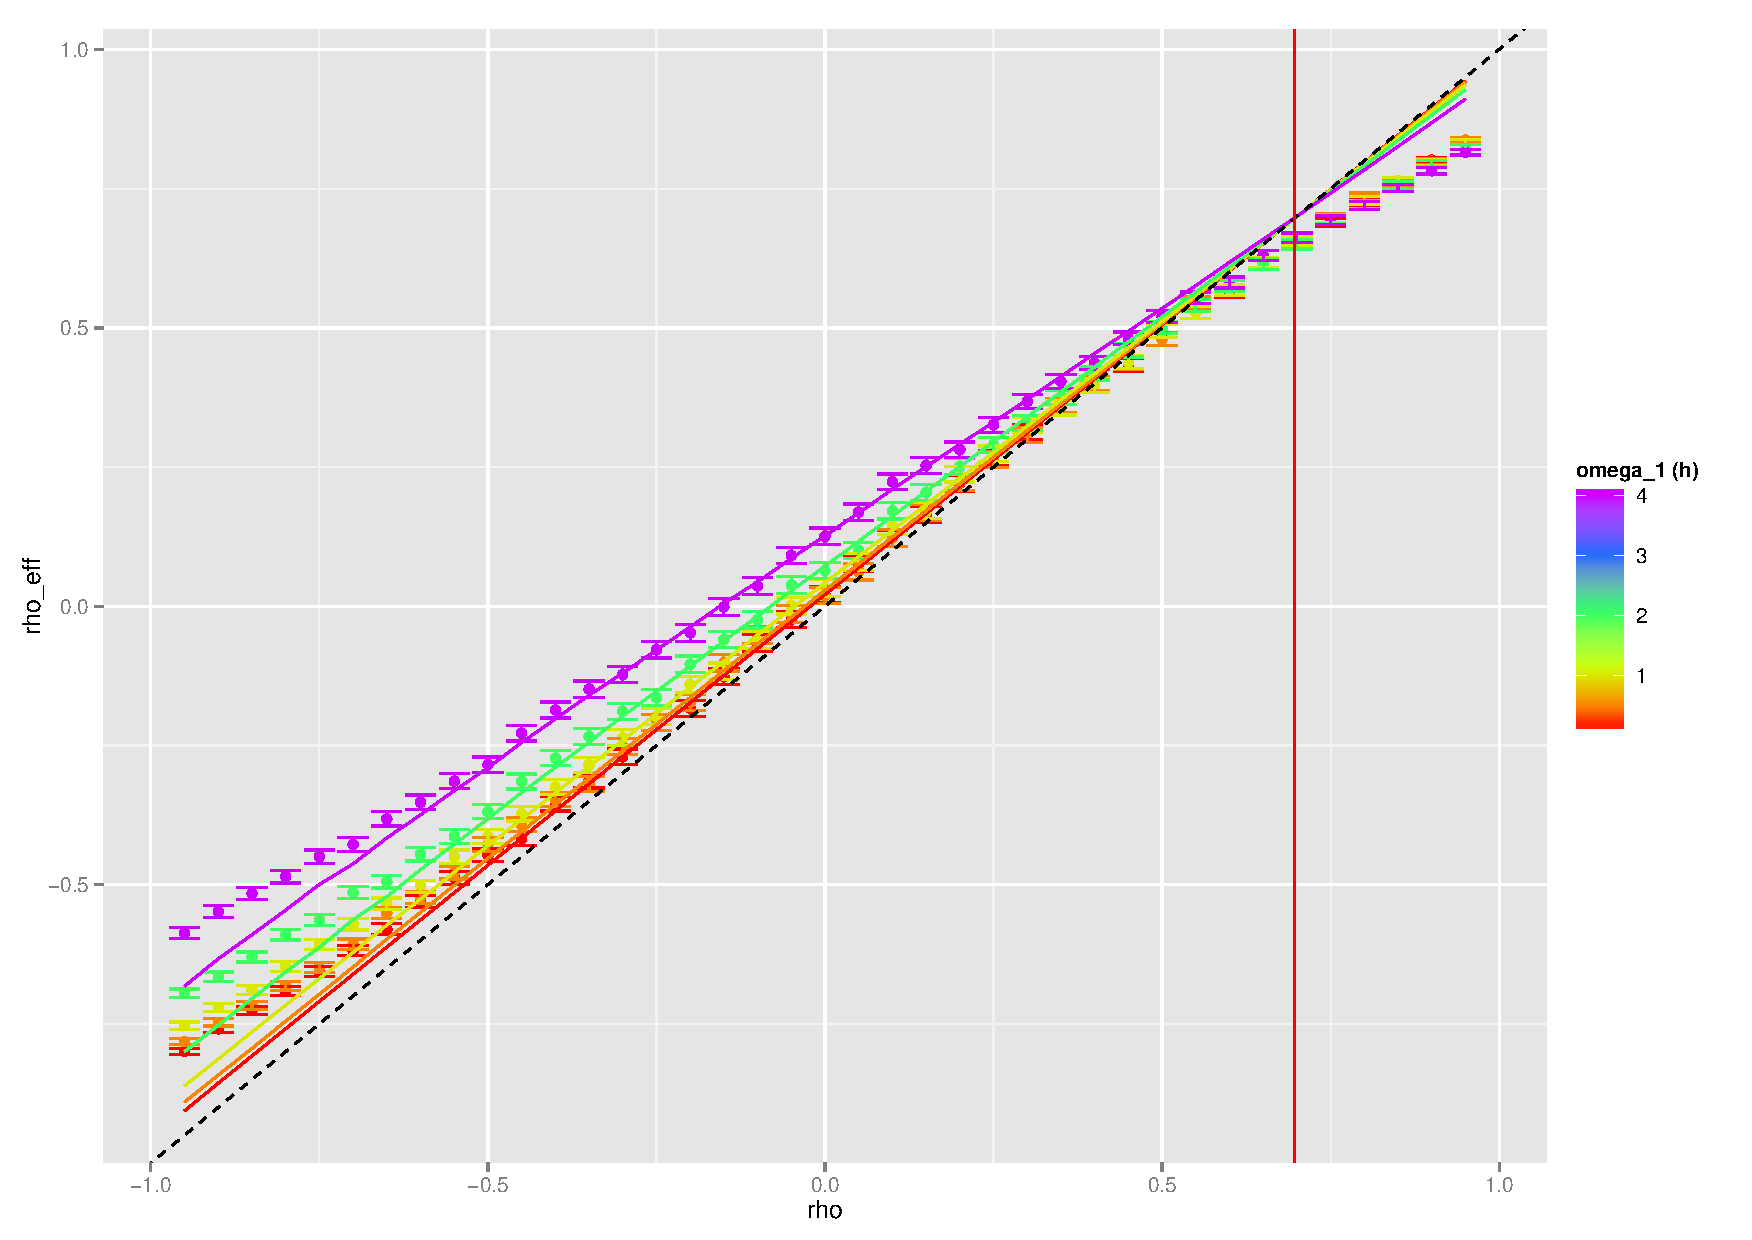
\includegraphics[width=0.8\textwidth,height=0.3\textheight]{figures/effectiveCorrs_withGoodTh_A4}
\caption{\small\textbf{Effective correlations obtained on synthetic data | } Dots represent estimated correlations on a synthetic dataset corresponding to 6 months between June and November 2015 (error-bars give 95\% confidence intervals obtained with standard Fisher method) ; scale color gives filtering frequency $\omega_1=10\textrm{min},30\textrm{min},1\textrm{h},2\textrm{h},4\textrm{h}$ ; solid lines give theoretical values for $\rho_e$ obtained by~\ref{eq:eff_corr} with estimated volatilities (dotted-line diagonal for reference) ; vertical red line position is the theoretical value such that $\rho = \rho_e$ with mean values for $\varepsilon_i$ on all points. We observe for high absolute correlations values a deviation from corrected values, what should be caused by non-verified independence and centered returns assumptions. Asymmetry is caused by the high value of $\rho_0 \simeq 0.71$.}
\label{fig:effective_corrs}
\end{figure}
%%%%%%%%%%%%%%%%%%%


%%%%%%%%%%%%%%%%%%%
\begin{figure}[h!]
% figure : performance of arma2 as a function of expected correlation.
%\vspace{-0.7cm}
\centering
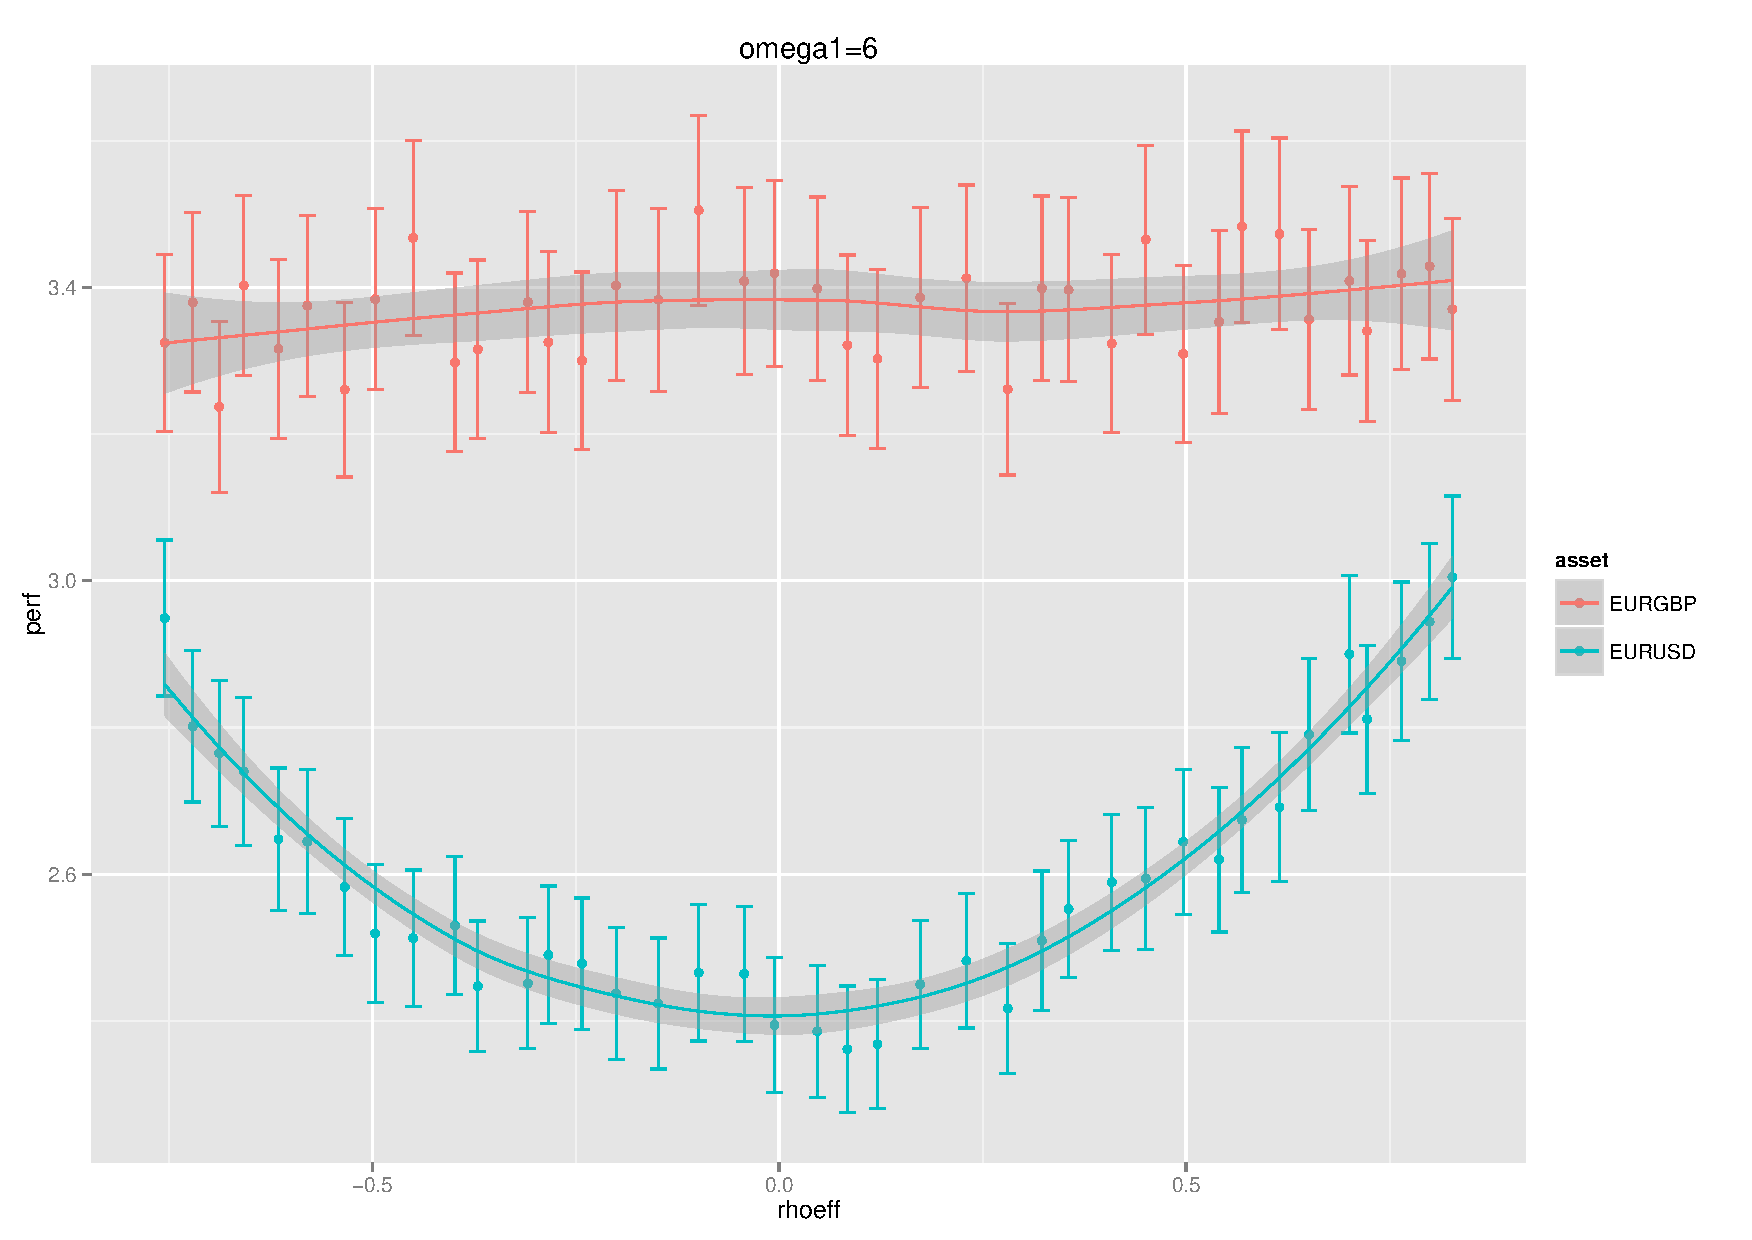
\includegraphics[width=0.48\textwidth,height=0.16\textheight]{figures/asset/pred_filt6}
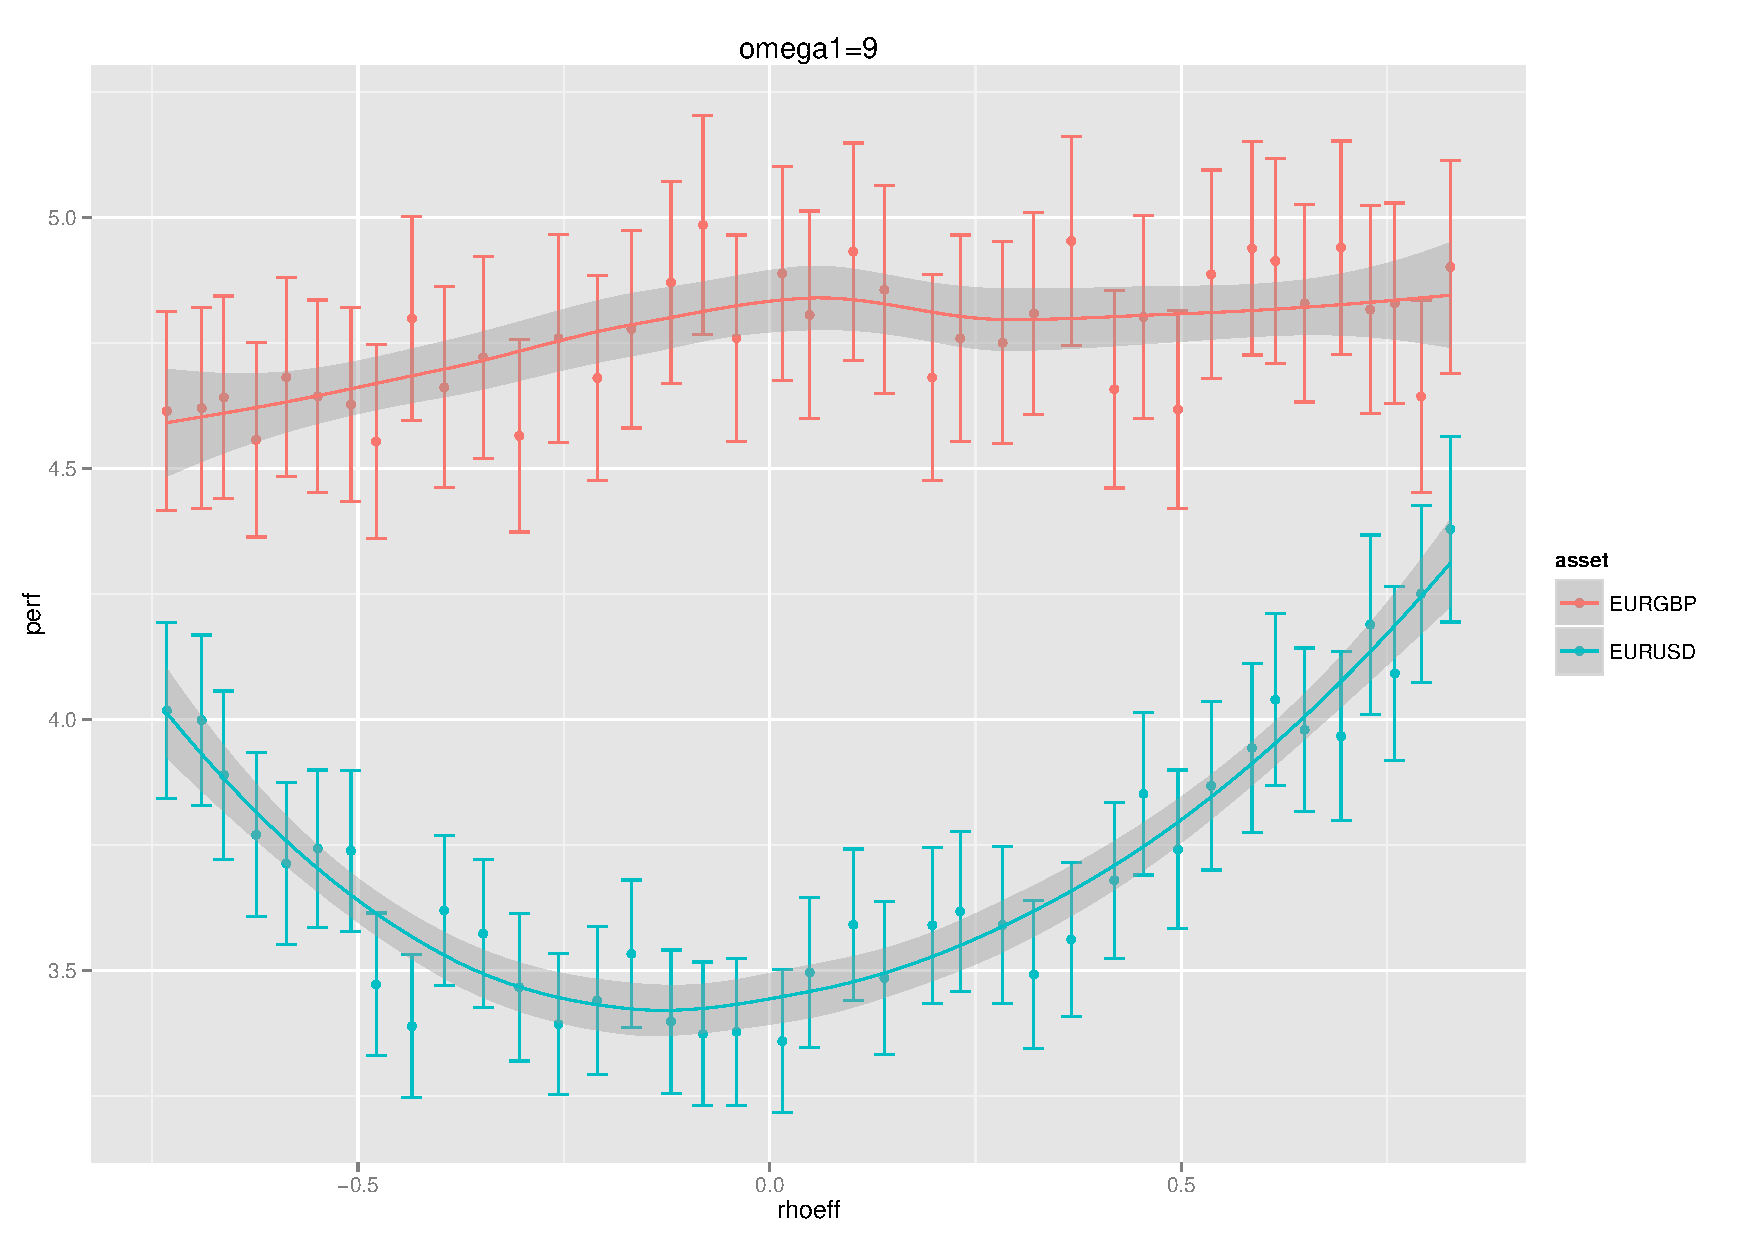
\includegraphics[width=0.48\textwidth,height=0.16\textheight]{figures/asset/pred_filt9}\\
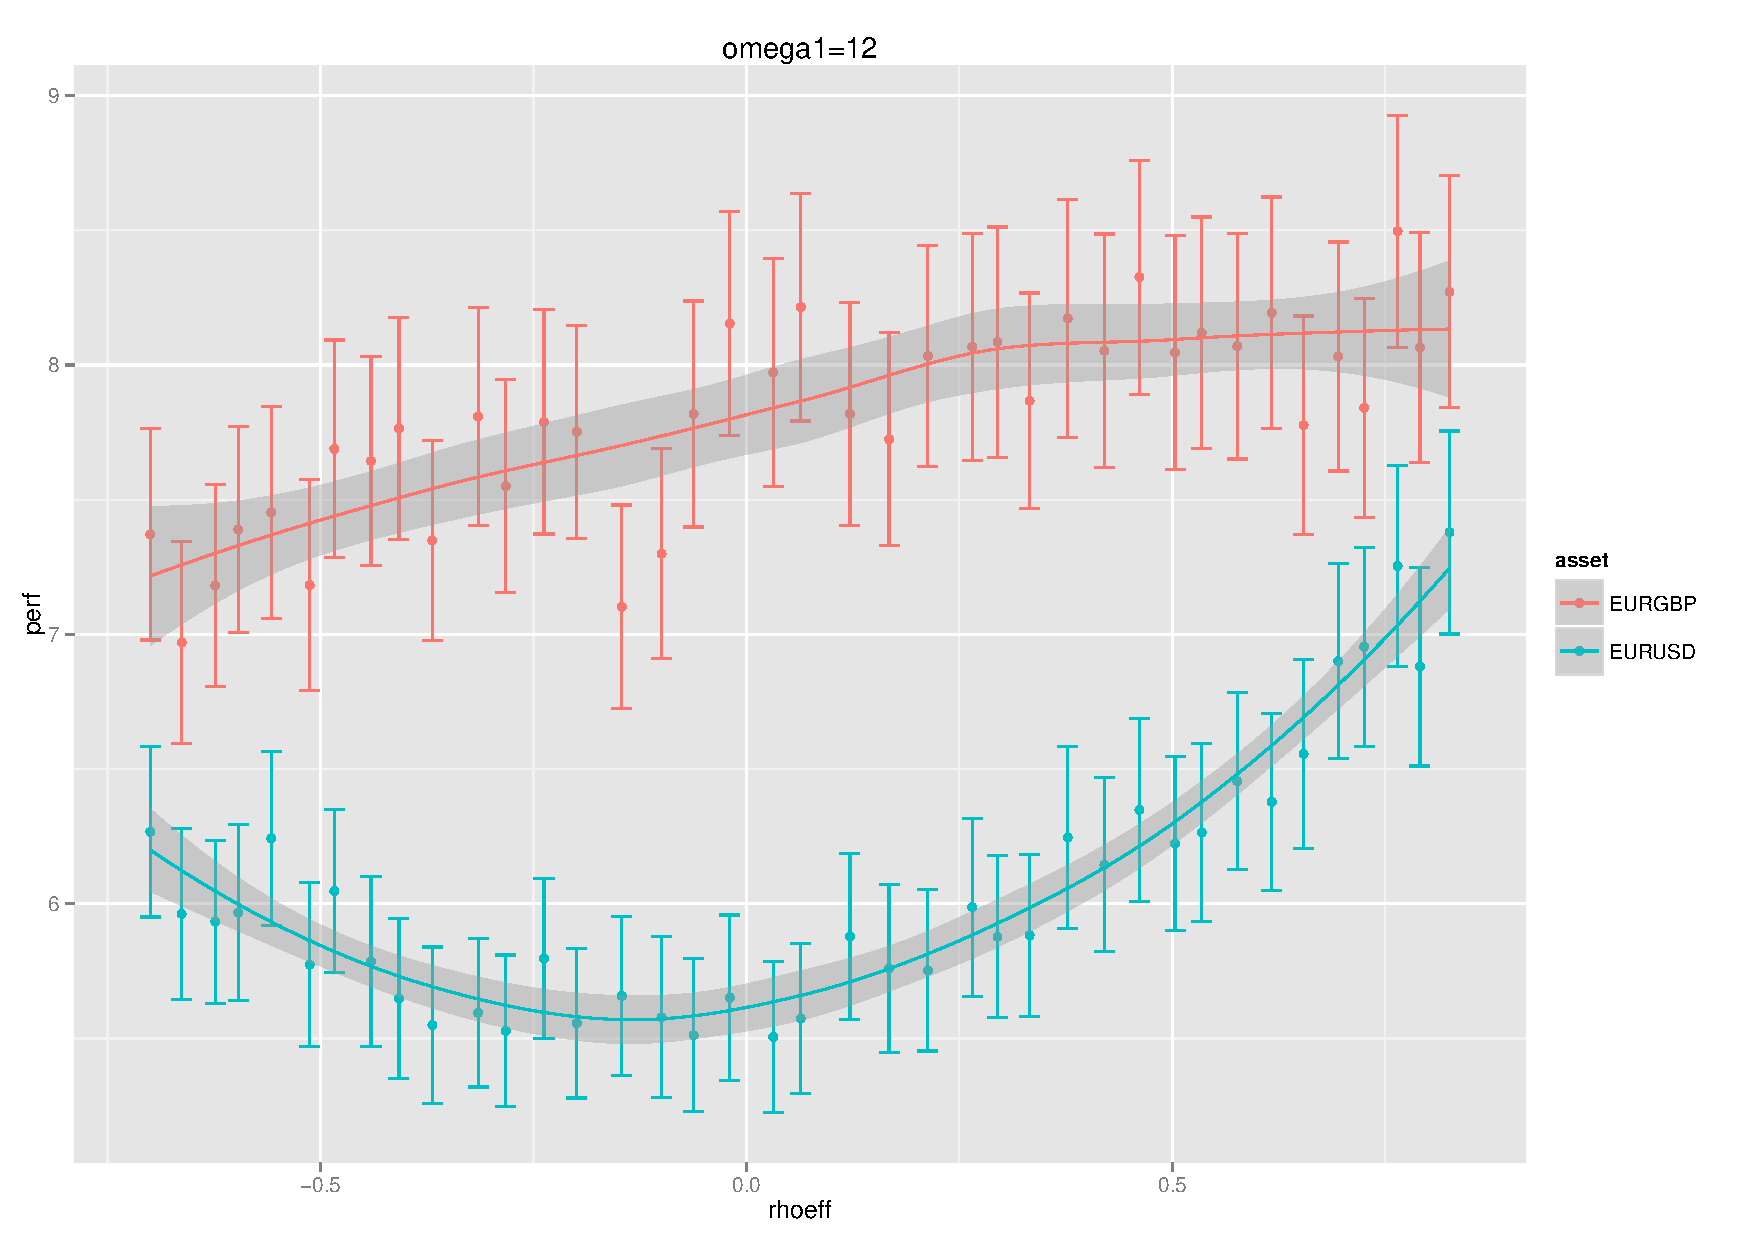
\includegraphics[width=0.48\textwidth,height=0.16\textheight]{figures/asset/pred_filt12}
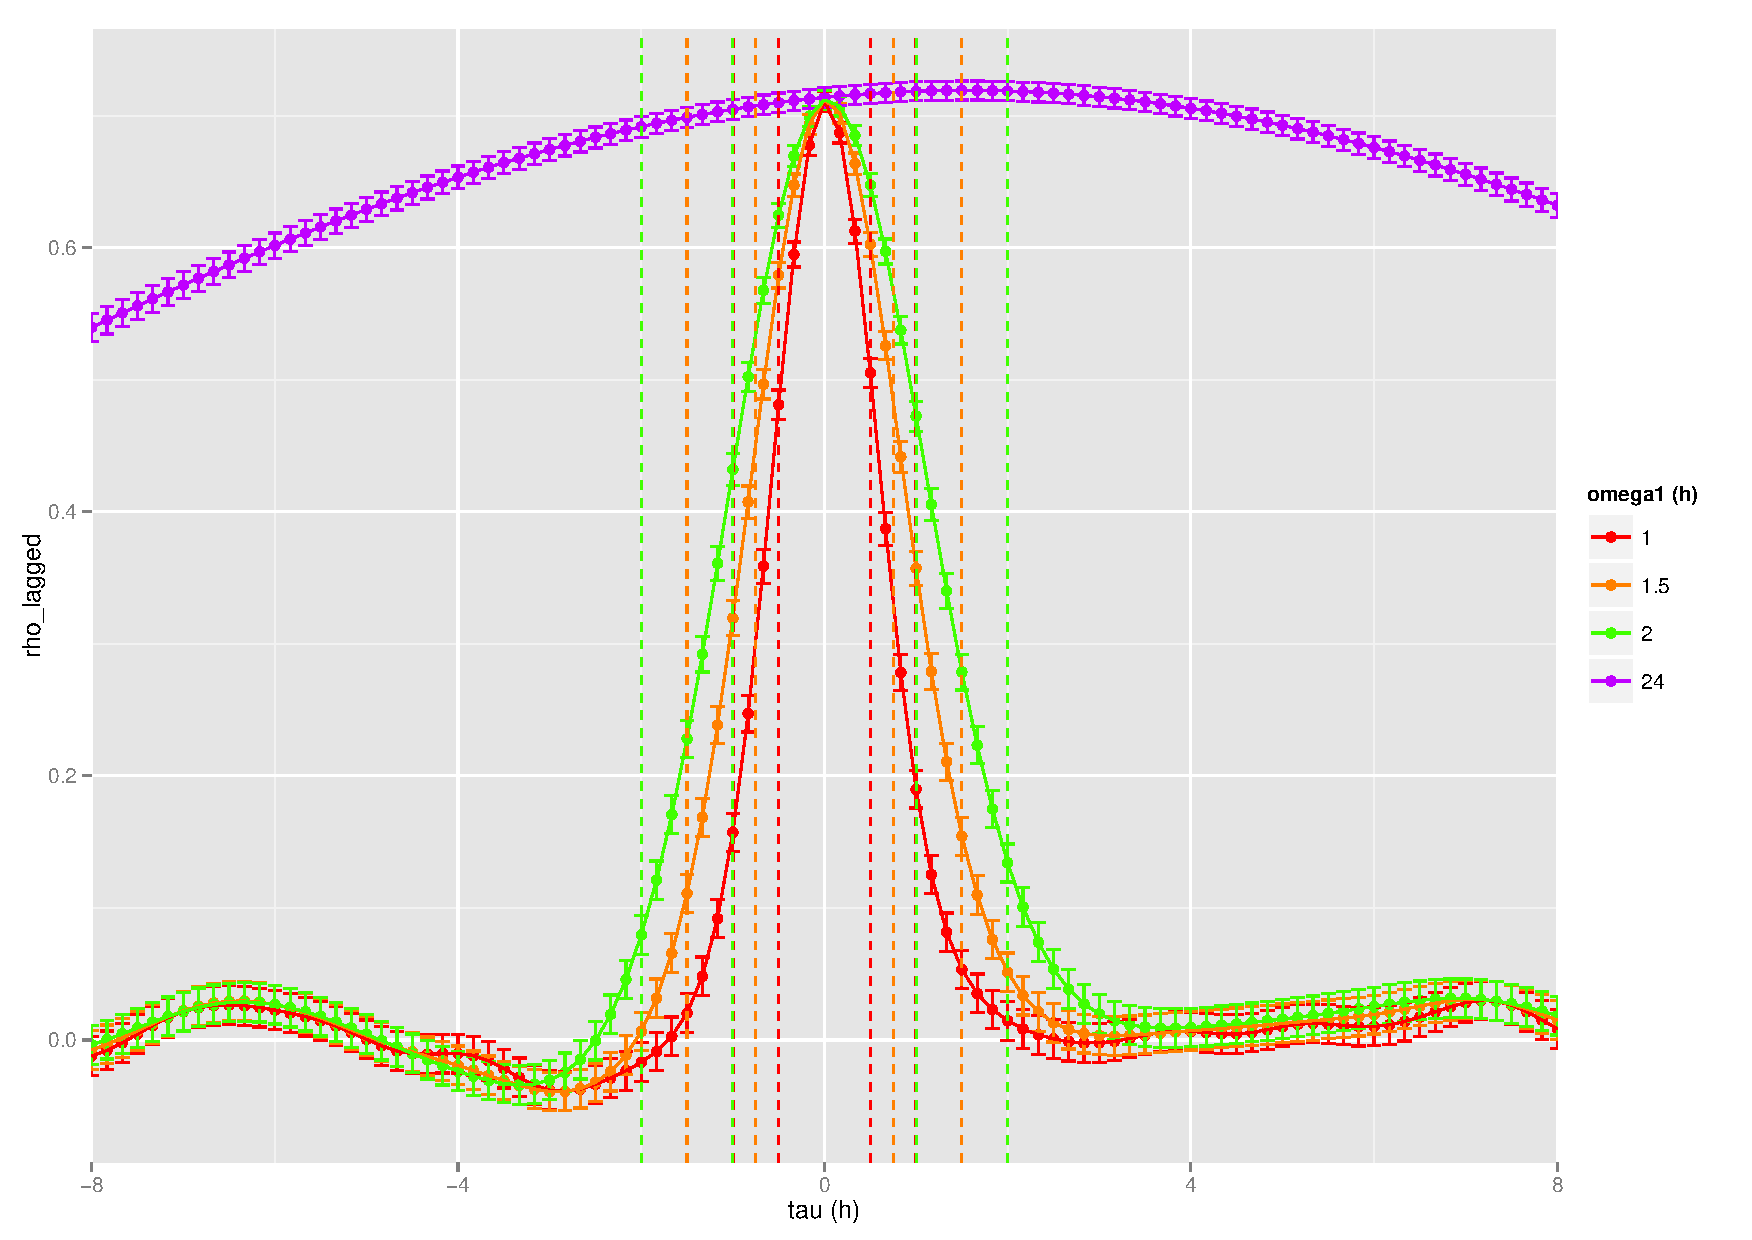
\includegraphics[width=0.48\textwidth,height=0.16\textheight]{figures/asset/lagged_corrs}
\caption{\small \textbf{Performance of a predictive model as a function of simulated correlations | } From left to right and top to bottom, three first graphs show for each asset the normalized performance of an ARMA model ($p=2,q=0$), defined as $\pi = \left(\frac{1}{T}\sum_t\left(\tilde{X}_i(t) - M_{\omega_1}\left[\tilde{X}_i\right](t)\right)^2 \right) / \sigma \left[ \tilde{X}_i \right]^2$ (95\% confidence intervals computed by $\pi = \bar{\pi} \pm (1.96\cdot \sigma [\pi])/\sqrt{T}$, local polynomial smoothing to ease reading). It is interesting to note the U-shape for EUR/USD, due to interference between components at different scales. Correlation between simulated noises deteriorates predictive power. The study of \emph{lagged correlations} (here $\rho [\Delta X_{\textrm{EURUSD}}(t),\Delta X_{\textrm{EURGBP}}(t-\tau)]$) on real data clarifies this phenomenon : fourth graph show an asymmetry in curves at any scale compared to zero lag $(\tau = 0)$ what leads fundamental components to increase predictive power for the dollar, amelioration then perturbed by correlations between simulated components. Dashed lines show time steps (in equivalent $\tau$ units) used by the ARMA at each scale, what allows to read the corresponding lagged correlation on fundamental component.}
\label{fig:model_perf}
\end{figure}
%%%%%%%%%%%%%%%%%%%




\newpage




%%%%%%%%%%%%%%%%%%%%%%
\subsection{Application : geographical data of density and network}


%%%%%%%%%%%%%%%%%%%%%%
\subsubsection{Context}


The use of synthetic data in geography is generally directed towards the generation of synthetic populations within agent-based models (mobility, \emph{LUTI} models)~\cite{pritchard2009advances}. We can make a weak link with some Spatial Analysis techniques. The extrapolation of a continuous spatial field from a discrete spatial sample through a kernel density estimation for example can be understood as the creation of a synthetic dataset (even if it is not generally the initial view, as in Geographically Weighted Regression~\cite{brunsdon1998geographically} in which variable size kernels do not interpolate data \emph{stricto sensu} but extrapolate abstract variables representing interaction between explicit variables). In the field of modeling in quantitative geography, \emph{toy-models} or hybrid models require a consistent initial spatial configuration. A set of possible initial configurations becomes a synthetic dataset on which the model is tested. The first Simpop model~\cite{sanders1997simpop}, precursor of a large family of models later parametrized with real data, could enter that frame but was studied on an unique synthetic spatialization. Similarly underlined was the difficulty to generate an initial transportation infrastructure in the case of the SimpopNet model~\cite{schmitt2014modelisation} although it was admitted as a cornerstone of knowledge on the behavior of the model. A systematic control of spatial configuration effects on the behavior of simulation models was only recently proposed~\cite{cottineau2015revisiting}, approach that can be interpreted as a statistical control on spatial data. The aim is to be able to distinguish proper effects due to intrinsic model dynamics from particular effects due to the geographical structure of the case study. Such results are essential for the validation of conclusions obtained with modeling and simulation practices in quantitative geography.

%En géographie, l'utilisation de données synthétiques est plus généralement axée vers l'utilisation de population synthétiques au sein de modèles basés agents (mobilité, modèles \emph{LUTI})~\cite{pritchard2009advances}. On peut également citer des méthodes d'analyse spatiales qui s'en rapprochent : par exemple, l'extrapolation d'un champ spatial continu à partir d'un échantillon discret, par une estimation par noyaux par exemple, peut être compris comme la génération d'un jeu de données synthétiques (même si ce n'est pas le point de vue initial, comme pour la Regression Géographique Pondérée~\cite{brunsdon1998geographically}, dans laquelle les noyaux de taille variables n'interpolent pas des données au sens propre mais extrapolent des variables abstraites représentant l'interaction entre variables explicites). Dans le domaine de la modélisation en géographie quantitative, dans le cas de \emph{modèles jouets} ou de modèles hybrides, une configuration initiale cohérente est souvent essentielle : un ensemble de configurations initiales possibles est alors un jeu de données synthétiques sur lesquelles le modèle est testé : le premier modèle Simpop~\cite{sanders1997simpop}, pionnier d'une famille de modèles par la suite paramétrisés par des données réelles, pourrait rentrer dans ce cadre mais était lancé sur une spatialisation synthétique unique. De même, il a été souligné la difficulté de générer une configuration initiale pour une infrastructure de transport dans le cas du modèle SimpopNet~\cite{schmitt2014modelisation}, alors qu'il s'agit un point essentiel dans la connaissance du comportement du modèle. Il a récemment été proposé de contrôler systématiquement les effets de la configuration spatiale sur le comportement de modèles de simulation spatialisés~\cite{cottineau2015revisiting}, méthodologie pouvant être interprétée comme un contrôle par données statistiques spatiales. L'enjeu est de pouvoir alors distinguer effets propres dus à la dynamique intrinsèque du modèle, d'effet particuliers dus à la structure géographique du cas d'application. Celui-ci est crucial pour la validation des conclusions issues des pratiques de modélisation et simulation en géographie quantitative.


%%%%%%%%%%%%%%%%%%%%%%
\subsubsection{Formalization}

We propose in our case to generate territorial systems summarized in a simplified way as a spatial population density $d(\vec{x})$ and a transportation network $n(\vec{x})$. Correlations we aim to control are correlations between urban morphological measures and network measures. The question of interactions between territories and networks is already well-studied~\cite{offner1996reseaux} but stays highly complex and difficult to quantify~\cite{offner1993effets}. A dynamical modeling of implied processes should shed light on these interactions (\cite{bretagnolle:tel-00459720}, p. 162-163). We develop in that frame a \emph{simple} coupling (i.e. without any feedback loop) between a density distribution model and a network morphogenesis model.

%Dans notre cas, nous proposons de générer des systèmes de villes représentés par une densité spatiale de population $d(\vec{x})$ et la donnée d'un réseau de transport $n(\vec{x})$, représenté de façon simplifiée, pour lesquels on serait capable de contrôler les correlations entre mesures morphologiques de la densité urbaine et caractéristiques du réseau. La question de l'interaction entre territoire et réseaux de transport est un sujet d'étude classique~\cite{offner1996reseaux} mais extrêmement complexe et difficile à quantifier~\cite{offner1993effets}. Une modélisation dynamique des processus impliqués devrait apporter des connaissances sur ces interactions (\cite{bretagnolle:tel-00459720}, p. 162-163). Dans ce cadre, nous développons un couplage \emph{simple} (c'est à dire sans boucle de rétroaction) entre un modèle de morphogenèse urbaine et un modèle de génération de réseau.


\paragraph{Density model}

We use a model $D$ similar to aggregation-diffusion models~\cite{batty2006hierarchy} to generate a discrete spatial distribution of population density. A generalization of the basic model is proposed in~\cite{raimbault2016calibration}, providing a calibration on morphological objectives (entropy, hierarchy, spatial auto-correlation, mean distance) against real values computed on the set of 50km sized grid extracted from european density grid~\cite{eurostat}. More precisely, the model proceeds iteratively the following way. An square grid of width $N$, initially empty, is represented by population $(P_i(t))_{1\leq i\leq N^2}$. At each time step, until total population reaches a fixed parameter $P_m$,
\begin{itemize}
\item total population is increased of a fixed number $N_G$ (growth rate), following a preferential attachment such that $\Pb{P_i(t+1)=P_i(t)+1|P(t+1)=P(t)+1}=\frac{(P_i(t)/P(t))^{\alpha}}{\sum(P_i(t)/P(t))^{\alpha}}$
\item a fraction $\beta$ of population is diffused to four closest neighbors is operated $n_d$ times
\end{itemize}



%L'utilisation d'un modèle $D$ type agrégation-diffusion~\cite{batty2006hierarchy} permet de générer une distribution discrete de densité. Dans \cite{raimbault2016calibration}, une généralisation de ce modèle est calibré pour des objectifs morphologiques (entropie, hiérarchie, auto-corrélation spatiale, distance moyenne) contre les valeurs réelles calculées sur l'ensemble des grilles de taille 50km extraites de la grille européenne de densité~\cite{eurostat}. Plus précisément, le modèle fonctionne de manière itérative de la façon suivante. Une grille initialement vide de côté $N$, est représentée par la données des populations $(P_i(t))_{1\leq i\leq N^2}$. A chaque pas de temps, jusqu'à ce que la population atteigne une valeur fixée $P_m$,
%\begin{itemize}
%\item la population totale $P(t)$ est augmentée d'un nombre fixé $N_G$ (taux de croissance), suivant un attachement préférentiel tel que $\Pb{P_i(t+1)=P_i(t)+1|P(t+1)=P(t)+1}=\frac{(P_i(t)/P(t))^{\alpha}}{\sum(P_i(t)/P(t))^{\alpha}}$
%\item une diffusion d'une fraction $\beta$ de la population aux 4 plus proches voisins est effectuée $n_d$ fois
%\end{itemize}


The two contradictory processes of urban concentration and urban sprawl are captured by the model, what allows to reproduce with a good precision a large number of existing morphologies.

%Les deux processus antagonistes de concentration et d'étalement urbain sont capturés par le modèle, ce qui permet de reproduire assez fidèlement un grand nombre de morphologies existantes.


\paragraph{Network model}


On the other hand, we are able to generate a planar transportation network by a model $N$, at a similar scale and given a density distribution. Because of the conditional nature to the density of the generation process, we will first have conditional estimators for network indicators, and secondly natural correlations between network and urban shapes should appear as processes are not independent. The nature and modularity of these correlations as a function of model parameters are still to determine by exploration of the coupled model.

%D'autre part, on est capable de générer par un modèle $N$ un réseau de transport planaire à une échelle équivalente, étant donné une distribution de densité. La génération du réseau étant conditionnée à la donnée de la densité, les estimateurs des indicateurs de réseau seront conditionnels d'une part, et d'autre part les formes urbaines et du réseau devraient nécessairement être corrélées, les processus n'étant pas indépendants. La nature et la modularité de ces correlations selon la variation des paramètres des modèles restent à déterminer par l'exploration du modèle couplé.

The heuristic network generation procedure is the following :
\begin{enumerate}
\item A fixed number $N_c$ of centers that will be first nodes of the network si distributed given density distribution, following a similar law to the aggregation process, i.e. the probability to be distributed in a given patch is $\frac{(P_i/P)^{\alpha}}{\sum (P_i/P)^{\alpha}}$. Population is then attributed according to Voronoi areas of centers, such that a center cumulates population of patches within its extent.
\item Centers are connected deterministically by percolation between closest clusters : as soon as network is not connected, two closest connected components in the sense of minimal distance between each vertices are connected by the link realizing this distance. It yields a tree-shaped network.
\item Network is modulated by potential breaking in order to be closer from real network shapes. More precisely, a generalized gravity potential between two centers $i$ and $j$ is defined by
\[
V_{ij}(d) = \left[ (1 - k_h) + k_h \cdot \left( \frac{P_i P_j}{P^2} \right)^{\gamma} \right]\cdot \exp{\left( -\frac{d}{r_g (1 + d/d_0)} \right)}
\]
where $d$ can be euclidian distance $d_{ij}=d(i,j)$ or network distance $d_N(i,j)$, $k_h \in [0,1]$ a weight to modulate role of populations, $\gamma$ giving shape of the hierarchy across population values, $r_g$ characteristic interaction distance and $d_0$ distance shape parameter.
\item A fixed number $K\cdot N_L$ of potential new links is taken among couples having greatest euclidian distance potential ($K=5$ is fixed).
\item Among potential links, $N_L$ are effectively realized, that are the one with smallest rate $\tilde{V}_{ij} = V_{ij}(d_N)/V_{ij}(d_{ij})$. At this stage only the gap between euclidian and network distance is taken into account : $\tilde{V}_{ij}$ does indeed not depend on populations and is increasing with $d_N$ at constant $d_{ij}$.
\item Planarity of the network is forced by creation of nodes at possible intersections created by new links.
\end{enumerate}



We insist on the fact that the network generation procedure is entirely heuristic and result of thematic assumptions (connected initial network, gravity-based link creation) combined with trial-and-error during first explorations. Other model types could be used as well, such biological self-generated networks~\cite{TeroAl10}, local network growth based on geometrical constraints optimization~\cite{barthelemy2008modeling}, or a more complex percolation model than the initial one that would allow the creation of loops for example. We could thus in the frame of a modular architecture, in which the choice between different implementations of a functional brick can be seen as a meta-parameter~\cite{cottineau2015incremental}, choose network generation function adapted to a specific need (as e.g. proximity to real data, constraints on output indicators, variety if generated forms, etc. ).

%Notons que la construction du modèle de génération est heuristique, et que d'autres types de modèles comme un réseau biologique auto-généré~\cite{TeroAl10}, une génération par optimisation locale de contraintes géométriques \cite{barthelemy2008modeling} ou un modèle de percolation plus complexe que celui utilisé, peuvent le remplacer. Ainsi, dans le cadre d'une architecture modulaire où le choix entre différentes implémentations d'une brique fonctionnelle peut être vue comme méta-paramètre~\cite{cottineau2015incremental}, on pourrait choisir la fonction de génération adaptée à un besoin donné (par exemple proximité à des données réelles, contraintes sur les relations entre indicateurs de sortie, variété de formes générées, etc.).


% TODO :: must do a computatonal benchmark for various network generation models ; calibrated on real data.

\paragraph{Parameter space}

Parameter space for the coupled model\footnote{Weak coupling allows to limit the total number of parameters as a strong coupling would involve retroaction loops and consequently associated parameters to determine their structure and intensity. In order to diminish it, an integrated model would be preferable to a strong coupling, what is slightly different in the sense where it is not possible in the integrated model to freeze one of the subsystems to obtain a model of the other subsystem that would correspond to the non-coupled model.} is constituted by density generation parameters $\vec{\alpha}_D = (P_m/N_G , \alpha,\beta , n_d)$ (we study for the sake of simplicity the rate between population and growth rate instead of both varying, i.e. the number of steps needed to generate the distribution) and network generation parameters $\vec{\alpha}_N=(N_C,k_h,\gamma , r_g , d_0)$. We denote $\vec{\alpha} = (\vec{\alpha}_D,\vec{\alpha}_N)$. 

%L'espace des paramètres du modèle couplé\footnote{Le couplage faible permet de limiter le nombre total de paramètres puisqu'un couplage fort incluant des boucles de retroaction comprendrait nécessairement des paramètres supplémentaires pour régler la forme et l'intensité de celles-ci. Pour espérer le diminuer, il faudrait concevoir un modèle intégré, ce qui est différent d'un couplage fort dans le sens où il n'est pas possible de figer l'un des sous-systèmes pour obtenir un modèle de l'autre correspondant au modèle non-couplé.} est constitué des paramètres de génération de densité $\vec{\alpha}_D = (P_m/N_G , \alpha,\beta , n_d)$ (on s'intéresse pour simplifier au rapport entre population et taux de croissance, i.e. le nombre d'étapes nécessaires pour générer) et des paramètres de génération de réseau $\vec{\alpha}_N=(N_C,k_h,\gamma , r_g , d_0)$. On notera $\vec{\alpha} = (\vec{\alpha}_D,\vec{\alpha}_N)$.


% TODO :: these notion of weak / strong coupling are not enough developed or reference-based. ---> find it in literature ? not sure exists like that. --> integarte it in theoretical paper ? or separate working paper.

\paragraph{Indicators}

Urban form and network structure are quantified by numerical indicators in order to modulate correlations between these. Morphology is defined as a vector $\vec{M}=(r,\bar{d},\varepsilon,a)$ giving spatial auto-correlation (Moran index), mean distance, entropy and hierarchy (see~\cite{le2015forme} for a precise definition of these indicators). Network measures $\vec{G} = (\bar{c},\bar{l},\bar{s},\delta)$ are with network denoted $(V,E)$
\begin{itemize}
\item Mean centrality $\bar{c}$ defined as average \emph{betweeness-centrality} (normalized in $[0,1]$) on all links.
\item Mean path length $\bar{l}$ given by $\frac{1}{d_m}\frac{2}{|V|\cdot (|V|-1)}\sum_{i<j}d_N(i,j)$ with $d_m$ normalization distance taken here as world diagonal $d_m=\sqrt{2}N$.
\item Mean network speed~\cite{banos2012towards} which corresponds to network performance compared to direct travel, defined as $\bar{s} = \frac{2}{|V|\cdot (|V|-1)}\sum_{i<j}{\frac{d_{ij}}{d_N(i,j)}}$.
\item Network diameter $\delta = \max_{ij}d_N(i,j)$.
\end{itemize}


%On quantifie la forme urbaine et la forme du réseau, dans le but de moduler la corrélation entre ces indicateurs. La forme est définie par un vecteur $\vec{M}=(r,\bar{d},\varepsilon,a)$ donnant auto-corrélation spatiale (indice de Moran), distance moyenne, entropie, hiérarchie (voir~\cite{le2015forme} pour une définition précise de ces indicateurs). Les mesures de la forme du réseau $\vec{G} = (\bar{c},\bar{l},\bar{s},\delta)$ sont, avec le réseau noté $(V,E)$,


\paragraph{Covariance and correlation}

We study the cross-correlation matrix $\Covb{\vec{M}}{\vec{G}}$ between morphology and network. We estimate it on a set of $n$ realizations at fixed parameter values $(\vec{M}\left[D(\vec{\alpha})\right],\vec{G}\left[N(\vec{\alpha})\right])_{1\leq i\leq n}$ with standard unbiased estimator. We estimate correlation with associated Pearson estimator. 



%%%%%%%%%%%%%%%%%%%%%%
\subsubsection{Implementation}


Coupling of generative models is done both at formal and operational levels. We interface therefore independent implementations. The OpenMole software~\cite{reuillon2013openmole} for intensive model exploration offers for that the ideal frame thanks to its modular language allowing to construct \emph{workflows} by task composition and interfacing with diverse experience plans and outputs. For operational reasons, density model is implemented in \texttt{scala} language as an OpenMole \texttt{plugin}, whereas network generation is implemented in agent-oriented language \texttt{NetLogo}~\cite{wilensky1999netlogo} because of its possibilities for interactive exploration and heuristic model construction. Source code is available for reproducibility on project repository\footnote{at \texttt{https://github.com/JusteRaimbault/CityNetwork/tree/master/Models/Synthetic}}.


%Le couplage des modèles génératifs est effectué à la fois au niveau formel et au niveau opérationnel, c'est à dire qu'on fait interagir des implémentations indépendantes. Pour cela, le logiciel OpenMole~\cite{reuillon2013openmole} utilisé pour l'exploration intensive, offre le cadre idéal de par son langage modulaire permettant de construire des \emph{workflows} par composition de tâches à loisir et de les brancher sur divers plans d'expérience et sorties. Pour des raisons opérationnelles, le modèle de densité est implémenté en langage \texttt{scala} comme un \texttt{plugin} d'OpenMole, tandis que la génération de réseau est implémentée en langage basé-agent \texttt{NetLogo}~\cite{wilensky1999netlogo}, ce qui facilite l'exploration interactive et construction heuristique interactive. Le code source est disponible pour reproductibilité sur le dépôt du projet\footnote{à l'adresse \texttt{https://github.com/JusteRaimbault/CityNetwork/tree/master/Models/Synthetic}}.





%%%%%%%%%%%%%%
\begin{figure}

\begin{subfigure}[t]{0.35\linewidth}
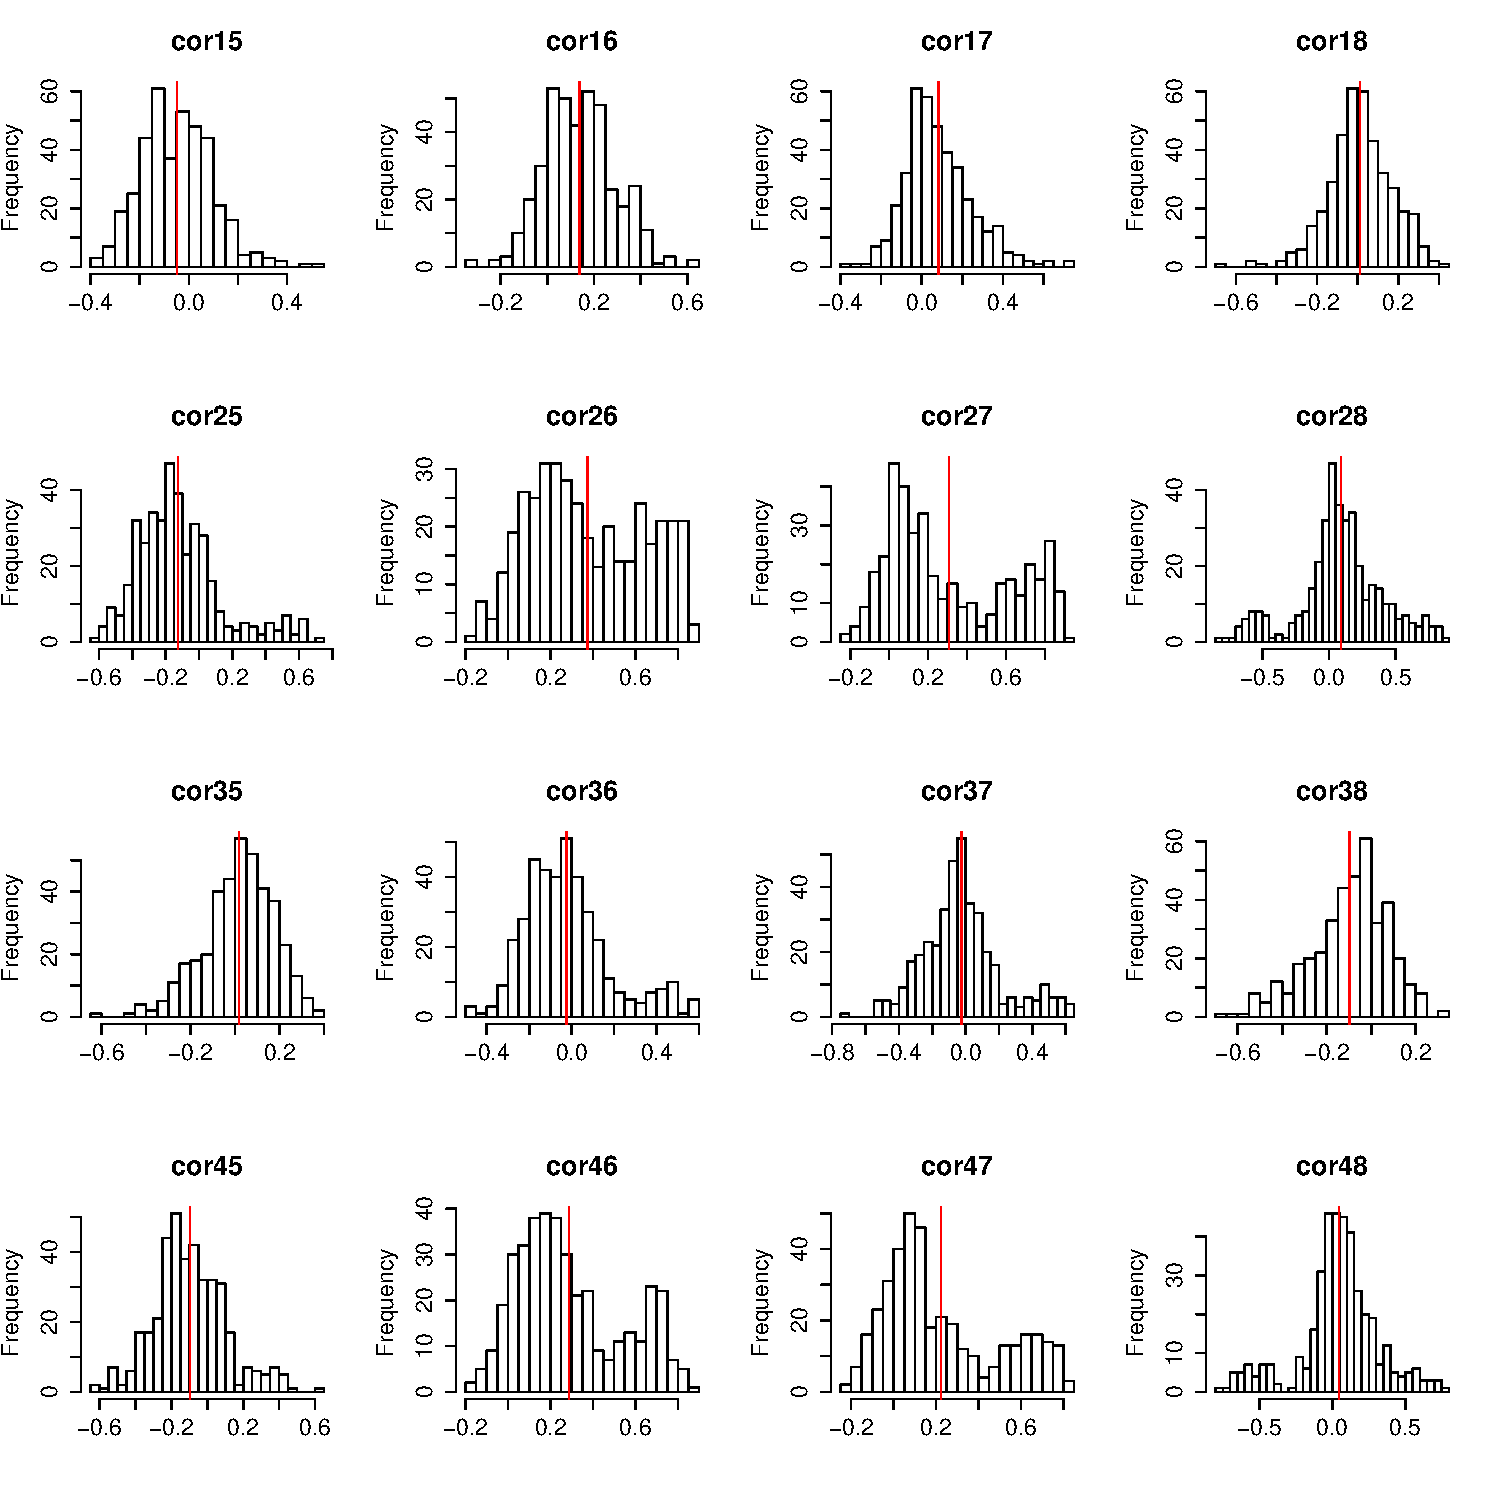
\includegraphics[width=\textwidth]{figures/hist_crossCorMat_breaks30}
\caption{}
\end{subfigure}
\begin{subfigure}[t]{0.23\linewidth}
\vspace{-6.5cm}
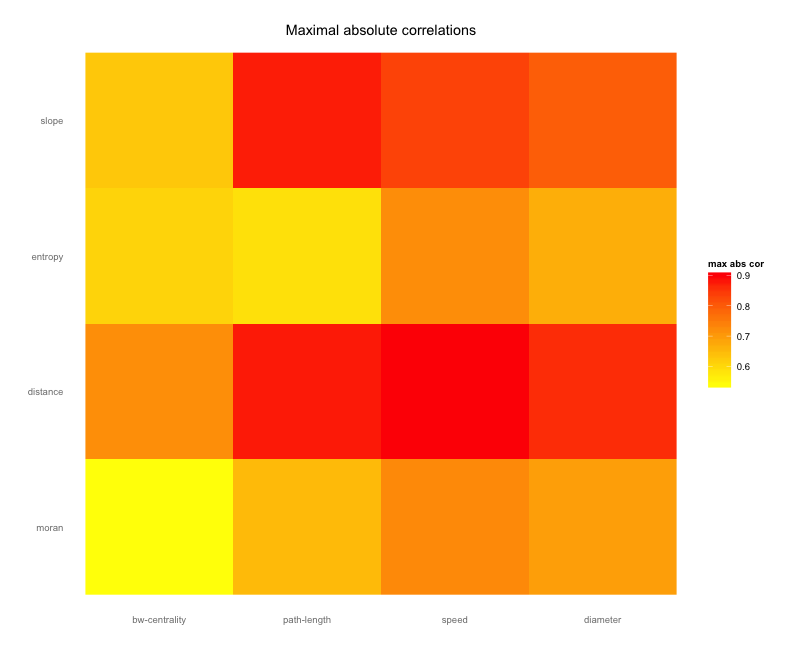
\includegraphics[width=\textwidth]{figures/heatmap_maxAbsCor}\\
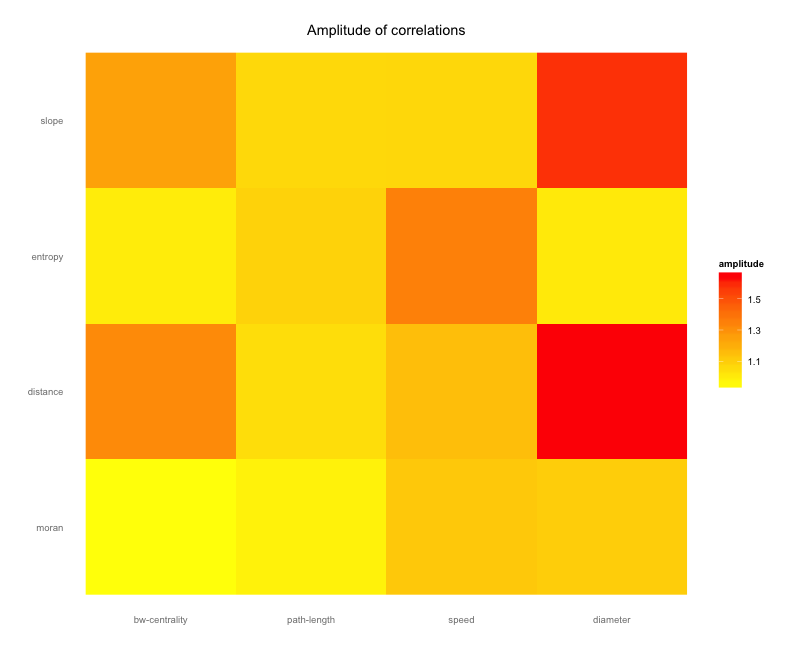
\includegraphics[width=\textwidth]{figures/heatmap_amplCor}
\caption{}
\end{subfigure}
\begin{subfigure}[t]{0.4\linewidth}
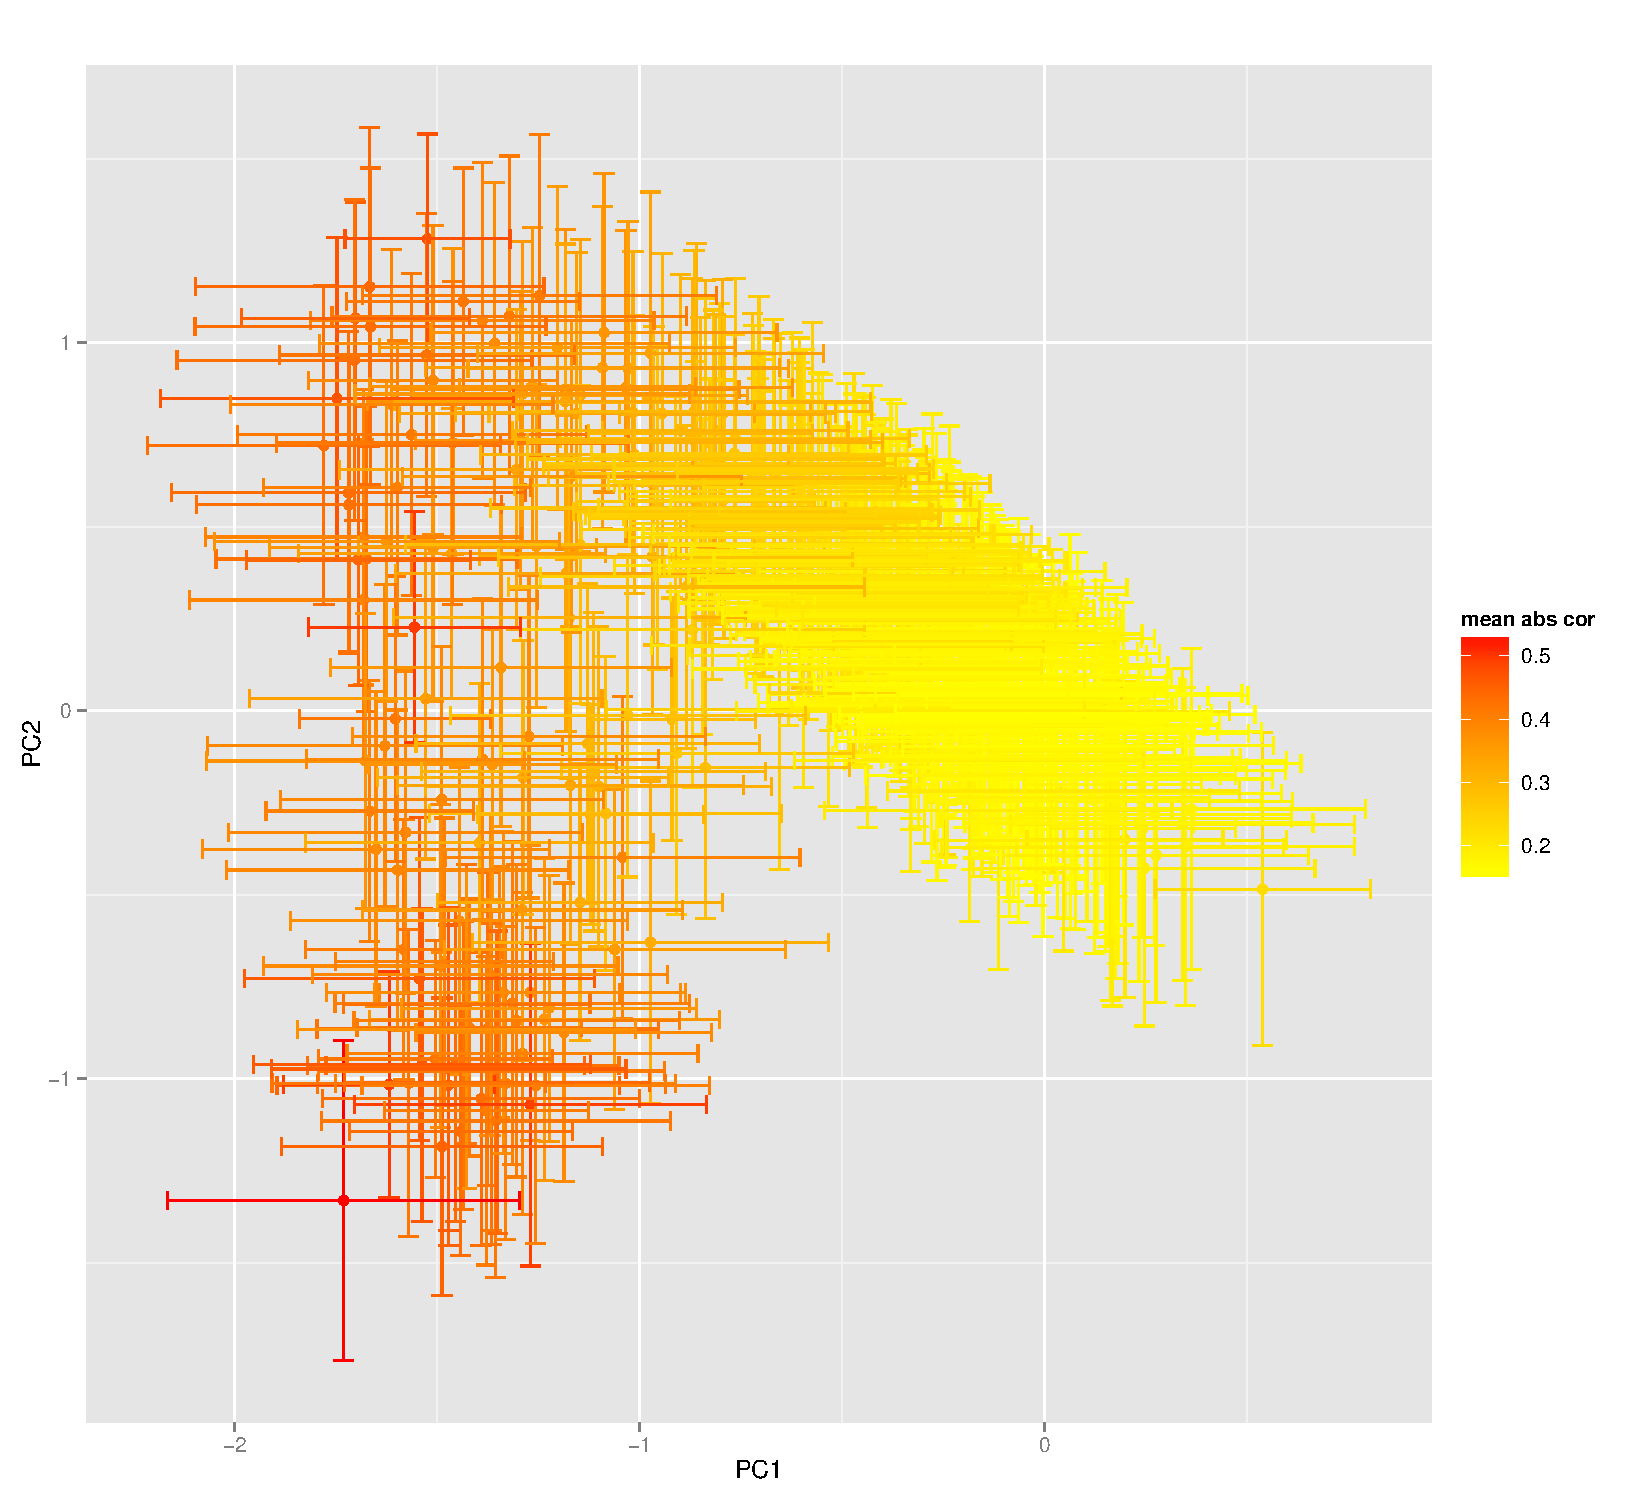
\includegraphics[width=\textwidth]{figures/pca_meanAbsCor_errorBars}
\caption{}
\end{subfigure}\\
\begin{subfigure}[t]{0.54\linewidth}
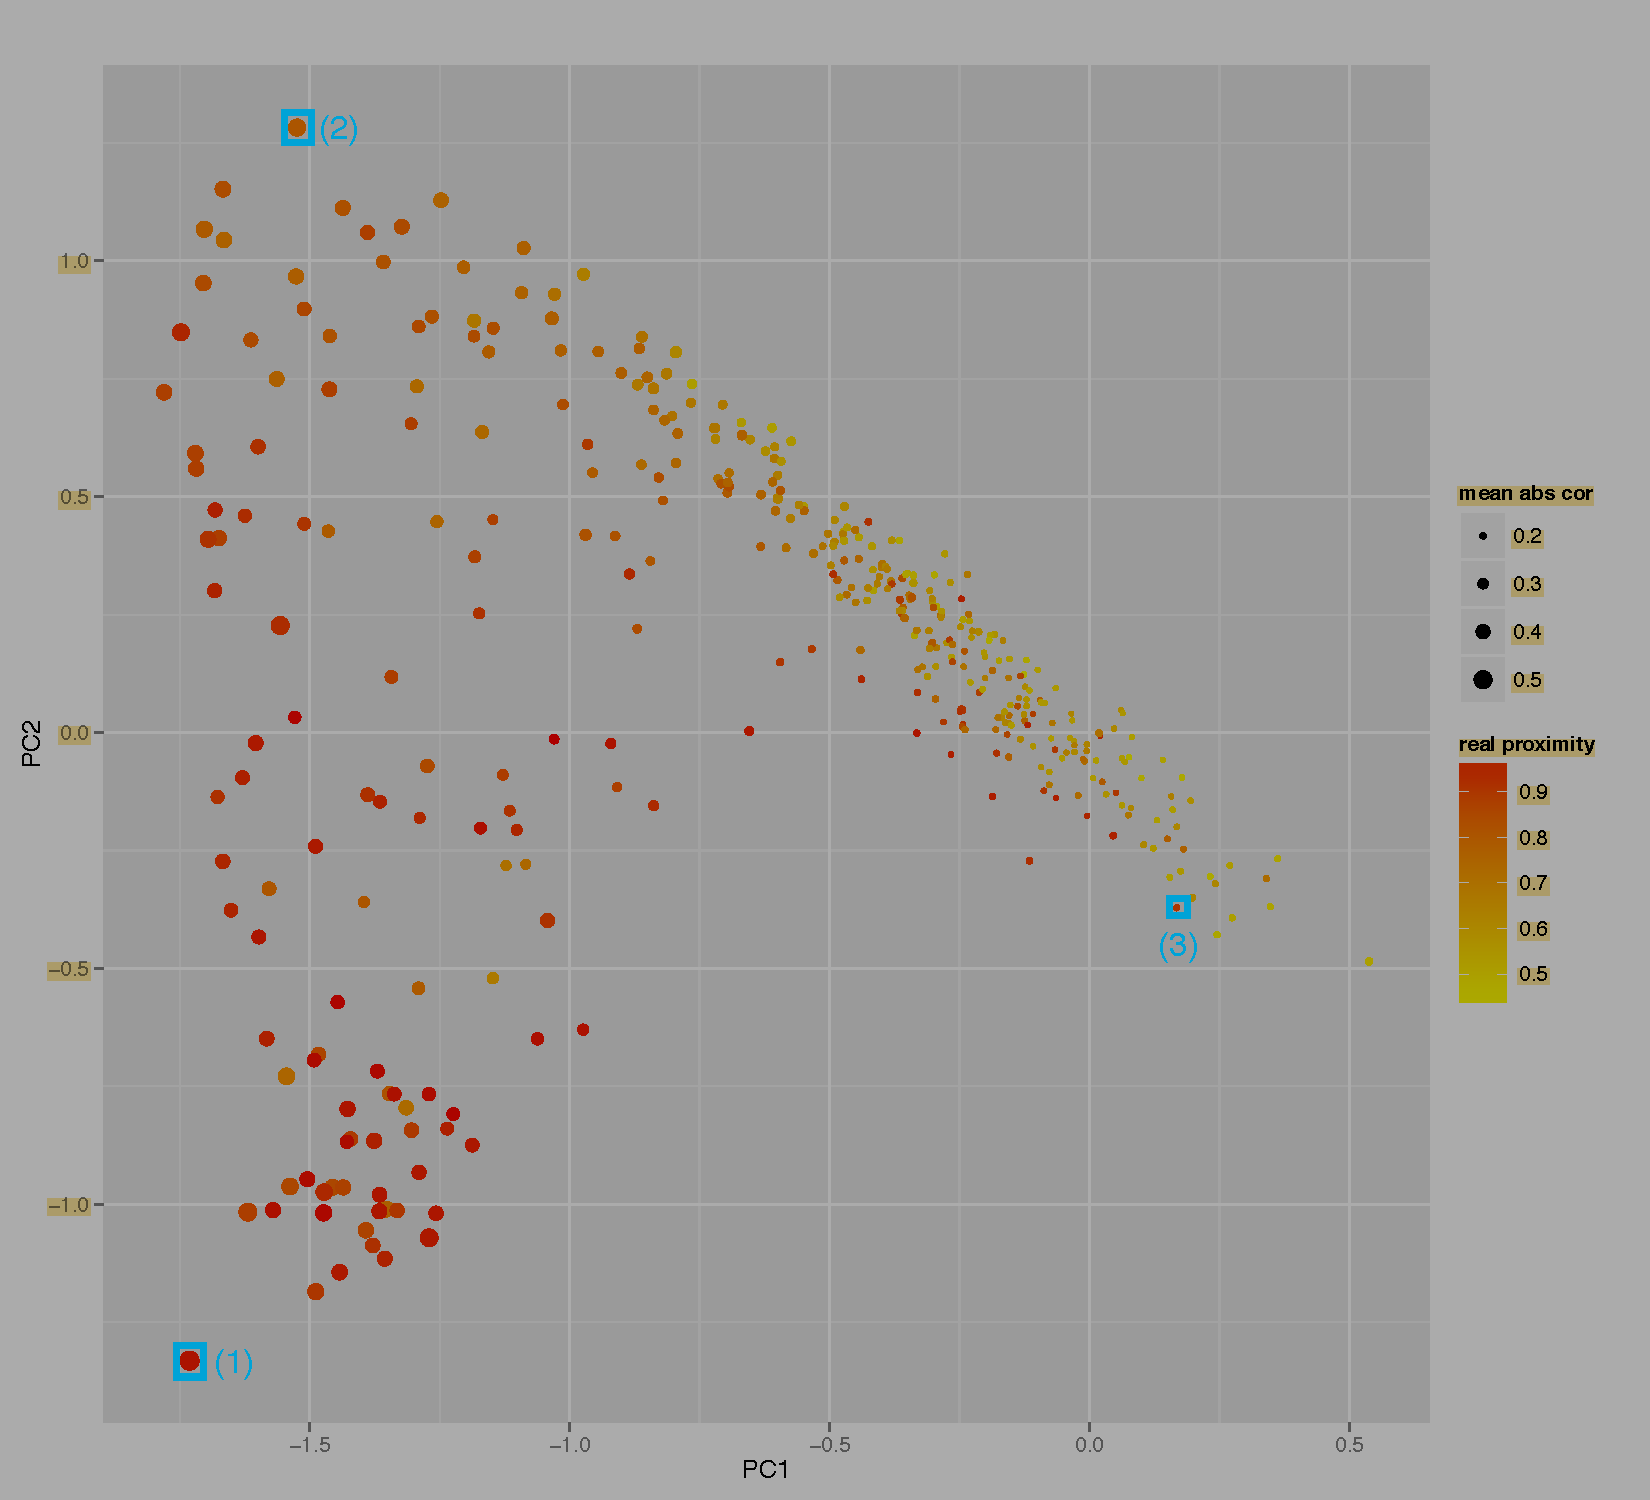
\includegraphics[width=\textwidth]{figures/pca_realDistCol_meanAbsCorSize_withSpecificPoints}
\caption{}
\end{subfigure}
\begin{subfigure}[t]{0.45\linewidth}
\vspace{-8.3cm}
   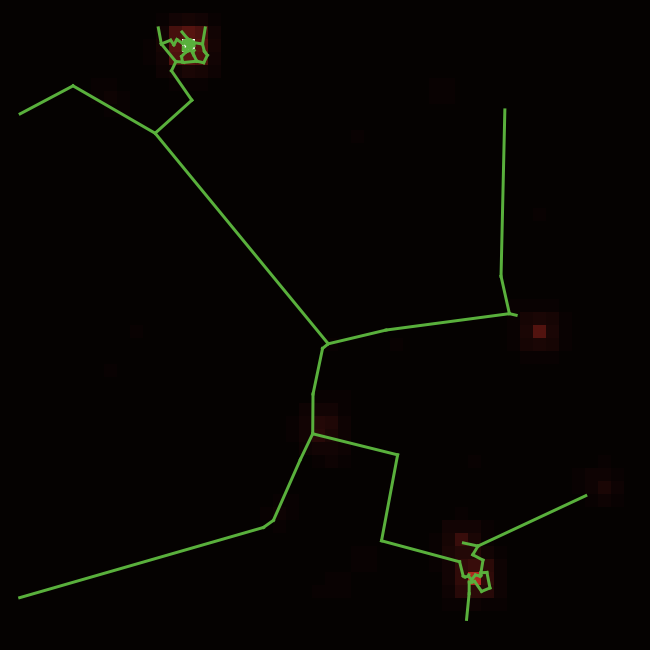
\includegraphics[width=0.49\textwidth]{figures/configs/1_param71861_seed0}
   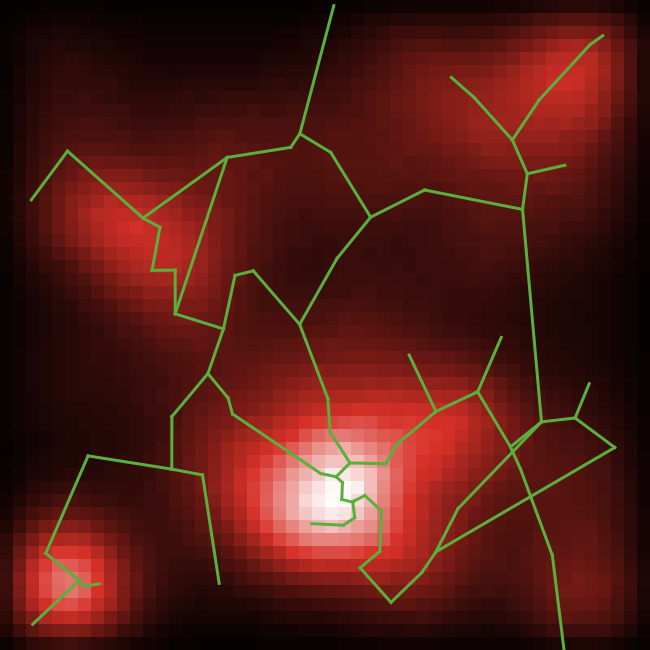
\includegraphics[width=0.49\textwidth]{figures/configs/2_param71913_seed10}\\
   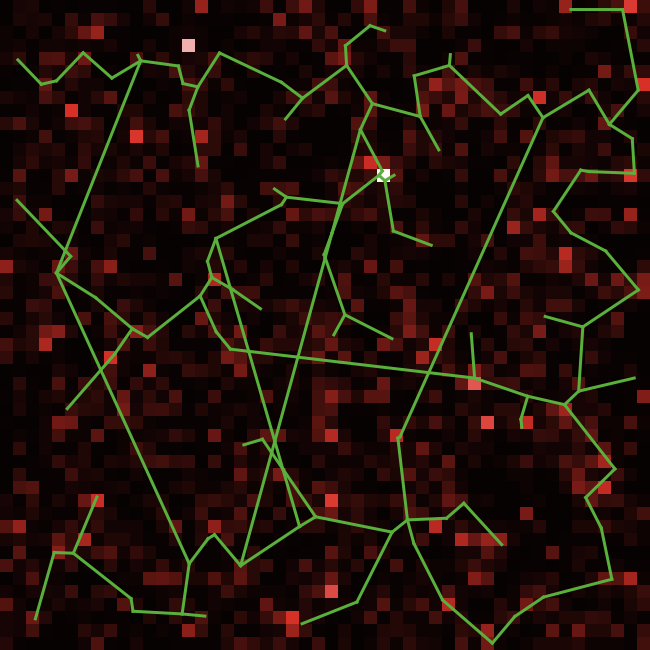
\includegraphics[width=0.49\textwidth]{figures/configs/3_param71918_seed0}
   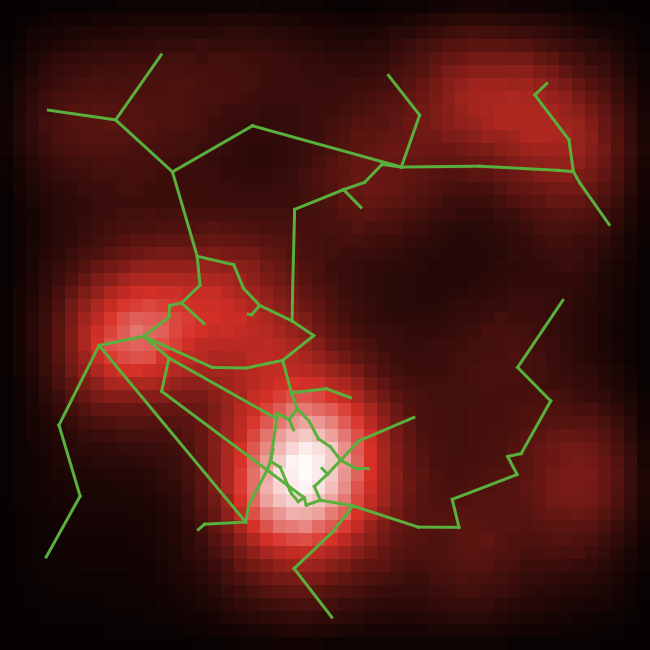
\includegraphics[width=0.49\textwidth]{figures/configs/4_param71945_seed0}
   \caption{}
\end{subfigure}

\caption{\small\textbf{Exploration of feasible space for correlations between urban morphology and network structure | } \textbf{(a)} Distribution of crossed-correlations between vectors $\vec{M}$ of morphological indicators (in numbering order moran index, mean distance, entropy, hierarchy) and $\vec{N}$ of network measures (centrality, mean path length, speed, diameter). \textbf{(b)} Heatmaps for amplitude of correlations, defined as $a_{ij}=\max_k{\rho_{ij}^{(k)}}-\min_k{\rho_{ij}^{(k)}}$ and maximal absolute correlation, defined as $c_{ij}=\max_k\left| \rho_{ij}^{k} \right|$. \textbf{(c)} Projection of correlation matrices in a principal plan obtained by Principal Component Analysis on matrix population (cumulated variances: PC1=38\%, PC2=68\%). Error bars are initially computed as 95\% confidence intervals on each matrix element (by standard Fisher asymptotic method), and upper bounds after transformation are taken in principal plan. Scale color gives mean absolute correlation on full matrices. \textbf{(d)} Representation in the principal plan, scale color giving proximity to real data defined as $1 - \min_r \norm{\vec{M}-\vec{M}_r}$ where $\vec{M}_r$ is the set of real morphological measures, point size giving mean absolute correlation. \textbf{(e)} Configurations obtained for parameters giving the four emphasized points in (d), in order from left to right and top to bottom. We recognize polycentric city configurations (2 and 4), diffuse rural settlements (3) and aggregated weak density area (1). See appendice for exhaustive parameter values, indicators and corresponding correlations. For example $\bar{d}$ is highly correlated with $\bar{l},\bar{s}$ ($\simeq$0.8) in (1) but not for (3) although both correspond to rural environments ; in the urban case we observe also a broad variability : $\rho[\bar{d},\bar{c}]\simeq 0.34$ for (4) but $\simeq-0.41$ for (2), what is explained by a stronger role of gravitation hierarchy in (2) $\gamma=3.9,k_h=0.7$ (for (4), $\gamma=1.07,k_h=0.25$), whereas density parameters are similar.}
\label{fig:densnwcor}
\end{figure}
%%%%%%%%%%%%%%






%%%%%%%%%%%%%%%%%%%%%%
\subsubsection{Results}

The study of density model alone is developed in~\cite{raimbault2016calibration}. It is in particular calibrated on European density grid data, on 50km width square areas with 500m resolution for which real indicator values have been computed on whole Europe. Furthermore, a grid exploration of model behavior yields feasible output space in reasonable parameters bounds (roughly $\alpha \in [0.5,2],N_G\in [500,3000], P_m \in [10^4,10^5],\beta\in [0,0.2], n_d \in \{ 1, \ldots , 4\}$). The reduction of indicators space to a two dimensional plan through a Principal Component Analysis (variance explained with two components $\simeq 80\%$) allows to isolate a set of output points that covers reasonably precisely real point cloud. It confirms the ability of the model to reproduce morphologically the set of real configurations.

%L'étude du modèle de densité seul est développée dans~\cite{raimbault2016calibration}. Il est notamment calibré sur les données de la grille européenne de densité, sur des zones de 50km de côté et de résolution 500m pour lesquelles les valeurs réelles des indicateurs ont été calculées pour l'ensemble de l'Europe. D'autre part, une exploration brutale du modèle permet d'estimer l'ensemble des sorties possibles dans des bornes raisonnables pour les paramètres (grossièrement $\alpha \in [0.5,2],N_G\in [500,3000], P_m \in [10^4,10^5],\beta\in [0,0.2], n_d \in \{ 1, \ldots , 4\}$). La réduction à un plan de l'espace des objectif par une Analyse en Composantes Principales (variance expliquée à deux composantes $\simeq 80\%$) permet d'isoler un nuage de points de sorties recouvrant assez fidèlement le nuage des points réels, ce qui veut dire que le modèle est capable de reproduire morphologiquement l'ensemble des configurations existantes.


% NOT NEEDED - TOO MUCH INFORMATION - ?
%%%%%%%%%%%%%%%%
%\begin{figure}
% figure : density example, exploration and calibration ?
%\end{figure}
%%%%%%%%%%%%%%%%

At given density, the conditional exploration of network generation model parameter space suggest a good flexibility on global indicators $\vec{G}$, together with good convergence properties. For a precise study of model behavior, see appendice giving regressions analysis capturing the behavior of coupled model. In order to illustrate synthetic data generation method, the exploration has been oriented towards the study of cross-correlations.


%A densité donnée, l'exploration de l'espace des paramètres du modèle de réseau suggèrent une assez bonne flexibilité sur des indicateurs globaux $\vec{G}$, ainsi que de bonnes propriétés de convergence. Pour une étude du comportement précis, voir l'appendice donnant les regressions traduisant le comportement du modèle couplé. Dans le but d'illustrer la méthode de génération de données synthétiques, l'exploration a été orientée vers l'étude des correlations.


Given the large relative dimension of parameter space, an exhaustive grid exploration is not possible. We use a Latin Hypercube sampling procedure with bounds given above for $\vec{\alpha}_D$ and for $\vec{\alpha}_N$, we take $N_C \in [50,120], r_g \in [1,100] , d_0 \in [0.1,10] , k_h \in [0,1] , \gamma \in [0.1,4],N_L\in [4,20]$. For number of model replications for each parameter point, less than 50 are enough to obtain confidence intervals at 95\% on indicators of width less than standard deviations. For correlations a hundred give confidence intervals (obtained with Fisher method) of size around 0.4, we take thus $n=80$ for experiments. Figure~\ref{fig:densnwcor} gives details of experiment results. Regarding the subject of correlated synthetic data generation, we can sum up the main lines as following :
\begin{itemize}
\item Empirical distributions of correlation coefficients between morphology and network indicators are not simple and some are bimodal (for example $\rho_{46}=\rho[r,\bar{l}]$  between Moran index and mean path length).
\item it is possible to modulate up to a relatively high level of correlation for all indicators, maximal absolute correlation varying between 0.6 and 0.9. Amplitude of correlations varies between 0.9 and 1.6, allowing a broad spectrum of values. Point cloud in principal plan has a large extent but is not uniform : it is not possible to modulate at will any coefficient as they stay themselves correlated because of underlying generation processes. A more refined study at higher orders (correlation of correlations) would be necessary to precisely understand degrees of freedom in correlation generation.
\item Most correlated points are also the closest to real data, what confirms the intuition and stylized fact of a strong interdependence in reality.
\item Concrete examples taken on particular points in the principal plan show that similar density profiles can yield very different correlation profiles.
\end{itemize}



%Etant donné la grande dimension relative de l'espace des paramètres, une exploration par grille exhaustive est impossible. On utilise un plan d'expérience par criblage (hypercube latin), avec les bornes indiquées ci-dessus pour $\vec{\alpha}_D$ et pour $\vec{\alpha}_N$, on a $N_C \in [50,120], r_g \in [1,100] , d_0 \in [0.1,10] , k_h \in [0,1] , \gamma \in [0.1,4],N_L\in [4,20]$. Concernant le nombre de réplications du modèle pour chaque valeur des paramètres, moins de 50 sont nécessaires pour obtenir sur les indicateurs des intervalles de confiance à 95\% de taille inférieure aux déviations standard. Pour les correlations, une centaine donne des IC (obtenus par méthode de Fisher) de taille moyenne 0.4, on fixe donc $n=80$ pour l'expérience. La figure~\ref{fig:densnwcor} donne le détail des résultats de l'exploration. On retiendra les résultats marquants suivants au regard de la génération de données synthétiques corrélées :
%\begin{itemize}
%\item les distributions empiriques des coefficients de correlations entre indicateurs de forme et indicateurs de réseaux ne sont pas simples, pouvant être bimodales (par exemple $\rho_{46}=\rho[r,\bar{l}]$ entre l'index de Moran et le chemin moyen).
%\item On arrive à générer un assez haut niveau de correlation pour l'ensemble des indicateurs, la correlation absolue maximale variant entre 0.6 et 0.9 ; l'amplitude varie quant à elle entre 0.9 et 1.6, ce qui permet un large spectre de valeurs. L'espace couvert dans un plan principal a une étendue certaine mais n'est pas uniforme : on ne peut pas moduler à loisir n'importe quel coefficients, ceux-ci étant liés par les processus de génération sous-jacent. Une étude plus fine aux ordres suivants (correlation des correlations) serait nécessaire pour cerner exactement la latitude dans la génération.
%\item les points les plus corrélés en moyenne sont également ceux les plus proches des données réelles, ce qui confirme l'intuition d'une forte interdépendance en réalité.
%\item Des exemples concrets pris sur des points particuliers distants dans le plan principal montre que des configurations de densité proches peuvent présenter des profils de correlations très différents.
%\end{itemize}



%%%%%%%%%%%%%%
%\begin{table}
%regression analysis of param influence on correlations
%  -> Appendice.
%\end{table}
%%%%%%%%%%%%%%




\subsubsection{Possible developments}


This case study could be refined by extending correlation control method. A precise knowledge of $N$ behavior (statistical distributions on an exhaustive grid of parameter space) conditional to $D$ would allow to determine $N^{<-1>} | D$ and have more latitude in correlation generation. We could also apply specific exploration algorithms to reach exceptional configurations realizing an expected correlation level, or at least to obtain a better knowledge of the feasible space of correlations~\cite{10.1371/journal.pone.0138212}.

%Il est possible de raffiner cette étude en étendant la méthode de contrôle des correlations. La connaissance très fine du comportement de $N$ (distribution statistiques sur une grille fine de l'espace des paramètres) conditionnée à $D$ devrait permettre de déterminer exhaustivement $N^{<-1>} | D$ et avoir plus de latitude dans la génération des correlations. On pourra également appliquer des algorithmes spécifiques d'exploration pour essayer atteindre des configurations exceptionnelles réalisant un niveau de corrélation voulu, ou au moins pour découvrir l'espace des correlations atteignables par la méthode de génération~\cite{10.1371/journal.pone.0138212}.




%%%%%%%%%%%%%%%%%%%%%%
\section{Discussion}
%%%%%%%%%%%%%%%%%%%%%%



%%%%%%%%%%%%%%%%%%%%%%
\subsection*{Scientific positioning}

% données hybrides au centre de la démarche d'exploration de modèle, analyse de sensitivité etc.

Our overall approach enters a particular epistemological frame. On the one hand the multidisciplinary aspect, and on the other hand the importance of empirical component through computational exploration methods, make this approach typical of Complex Systems science, as it is recalled by the roadmap for Complex Systems having a similar structure~\cite{2009arXiv0907.2221B}. It combines transversal research questions (horizontal integration of disciplines) with the development of heterogeneous multi-scalar approaches which encounter similar issues as the one we proposed to tackle (vertically integrated disciplines). The combination of empirical knowledge obtained from data mining, with knowledge obtained by modeling and simulation is generally central to the conception and exploration of multi-scalar heterogeneous models. Results presented here is an illustration of such an hybrid paradigm.

%Notre démarche s'inscrit dans un cadre épistémologique particulier. En effet, d'une part la volonté de multi-disciplinarité et d'autre part l'importance de la composante empirique couplée aux méthodes d'exploration computationelles, en font une approche typique des sciences de la complexité, comme le rappelle la structure de la feuille de route pour les systèmes complexes~\cite{2009arXiv0907.2221B} qui croise des grandes questions transversales aux disciplines à une intégration verticale de celles-ci, qui implique la construction de modèles multi-échelles hétérogènes présentant souvent les aspects précédent. Le croisement de connaissances empiriques issues de la fouille de données avec celles issues de la simulation est souvent central dans leur conception ou leur exploration, et les résultats présentés ici en sont un exemple typique pour le cas de l'exploration.



%%%%%%%%%%%%%%%%%%%%%%
\subsection*{Direct applications}


Starting from the second example which was limited to data generation, we propose examples of direct applications that should give an overview of the range of possibilities.

%En partant du deuxième exemple, qui s'est arrêté à la génération des données synthétiques, on peut proposer des pistes d'application directe qui donneront un aperçu de l'éventail des possibilités.

\begin{itemize}
\item Calibration of network generation component at given density, on real data for transportation network (typically road network given the shape of generated networks ; it should be straightforward to use OpenStreetMap open data\footnote{\texttt{https://www.openstreetmap.org}} that have a reasonable quality for Europe, at least for France~\cite{girres2010quality}, with however adjustments on generation procedure in order to avoid edge effects due its restrictive frame, for example by generating on an extended surface to keep only a central area on which calibration would be done) should theoretically allow to unveil parameter sets reproducing accurately existing configurations both for urban morphology and network shape. It could be then possible to derive a ``theoretical correlation'' for these, as an empirical correlation is according to some theories of urban systems not computable as a unique realization of stochastic processes is observed. Because of non-ergodicity of urban systems~\cite{pumain2012urban}, there are strong chances that involved processes are different across different geographical areas (or from an other point of view that they are in an other state of meta-parameters, i.e. in an other regime) and that their interpretation as different realizations of the same stochastic process makes no sense, the impossibility of covariation estimation following. By attributing a synthetic dataset similar to a given real configuration, we would be able to compute a sort of \emph{intrinsic correlation} proper to this configuration. As territorial configurations emerge from spatio-temporal interdependences between components of territorial systems, this intrinsic correlation emerges the same way, and its knowledge gives information on these interdependences and thus on relations between territories and networks.
\item As already mentioned, most of models of simulation need an initial state generated artificially as soon as model parametrization is not done completely on real data. An advanced model sensitivity analysis implies a control on parameters for synthetic dataset generation, seen as model meta-parameters~\cite{cottineau2015revisiting}. In the case of a statistical analysis of model outputs it provides a way to operate a second order statistical control.
\item We studied in the first example stochastic processes in the sense of random time-series, whereas time did not have a role in the second case. We can suggest a strong coupling between the two model components (or the construction of an integrated model) and to observe indicators and correlations at different time steps during the generation. In a dynamical spatial models we have because of feedbacks necessarily propagation effects and therefore the existence of lagged interdependences in space and time~\cite{pigozzi1980interurban}. It would drive our field of study towards a better understanding of dynamical correlations.
\end{itemize}


%\begin{itemize}
%\item La calibration de la composante de génération de réseau, à densité donnée, sur des données réelle de réseau de transport (typiquement routier vu les formes heuristiques obtenues, il devrait par exemple être aisé d'utiliser les données ouvertes d'OpenStreetMap\footnote{\texttt{https://www.openstreetmap.org}} qui sont de qualité raisonnable pour l'Europe, du moins pour la France~\cite{girres2010quality}, avec toutefois des ajustements à faire sur le modèle pour supprimer les effets de bord du à sa structure, par exemple en le faisant générer sur une surface étendue pour ne garder qu'une zone centrale sur laquelle la calibration aurait lieu) permettrait en théorie d'isoler un jeu de paramètres représentant fidèlement des situations existantes à la fois pour la forme urbaine et la forme du réseau. Il serait alors possible de dériver une ``correlation théorique'' pour celles-ci, étant donné qu'une correlation empirique n'est en théorie pas calculable puisqu'une seule instance des processus stochastiques est observée. Vu la non-ergodicité des systèmes urbains~\cite{pumain2012urban}, il y a de fortes chances pour que ces processus soient différents d'une zone géographique à l'autre (ou selon un autre point de vue qu'ils soient dans un autre état des meta-paramètres, dans un autre régime) et que leur interprétation en tant que réalisations d'un même processus stochastique n'ait aucun sens, entrainant l'impossibilité du calcul des covariations. En attribuant un jeu de données synthétiques similaire à une situation donnée, on serait capable de calculer une sorte de \emph{correlation intrinsèque} propre à la situation, qui émerge en fait en réalité des interdépendances temporelles des composantes. Connaitre celle-ci renseigne alors sur ces interdépendances, et donc sur les relations entre réseaux et territoires.
%\item Comme déjà évoqué, la plupart des modèles de simulation nécessitent un état initial, généré artificiellement à partir du moment où la paramétrisation n'est pas effectuée totalement à partir de données réelles. Une analyse de sensibilité avancée du modèle implique alors un contrôle sur les paramètres de génération du jeu de données synthétique, vu comme méta-paramètre du modèle~\cite{cottineau2015revisiting}. Dans le cas d'une analyse statistique des sorties du modèle, on est alors capable d'effectuer un contrôle statistique au second ordre.
%\item On a étudié des processus stochastiques dans le premier exemple, au sens de séries temporelles aléatoires, alors que le temps ne jouait pas de rôle dans le second. On peut suggérer un couplage fort entre les deux composantes du modèle (ou la construction d'un modèle intégré) et observer les indicateurs et correlations à différents pas de temps de la génération. Dans le cas d'une dynamique, de par les rétroactions, on a nécessairement des effets de propagation et donc l'existence d'interdépendances décalées dans l'espace et le temps~\cite{pigozzi1980interurban}, étendant le domaine d'étude vers une meilleure compréhensions des correlations dynamiques.
%\end{itemize}



%%%%%%%%%%%%%%%%%%%%%%
\subsection*{Generalization}

We were limited to the control of first and second moments of generated data, but we could imagine a theoretical generalization allowing the control of moments at any order. However, as shown by the geographical example, the difficulty of generation in a concrete complex case questions the possibility of higher orders control when keeping a consistent structure model and a reasonable number of parameters. The study of non-linear dependence structures as proposed in~\cite{chicheportiche2013nested} is in an other perspective an interesting possible development.

%On s'est limité au contrôle des premiers et second moments des données générées, mais il est possible d'imaginer une généralisation théorique permettant le contrôle des moments à un ordre arbitraire. Toutefois, la difficulté de génération dans un cas concret complexe, comme le montre l'exemple géographique, questionne la possibilité de contrôle aux ordres supérieurs tout en gardant un modèle à la structure cohérente et au nombre de paramètres relativement faibles. Par contre, l'étude de structures de dépendances non-linéaires comme celles utilisées dans~\cite{chicheportiche2013nested} est une piste de développement intéressante.

%%%%%%%%%%%%%%%%%%%%%%
%\subsection*{Autres domaines potentiels d'application}
% ideas of other fields where the generation can happen.
% -> not necessary, suggested in intro ?



%%%%%%%%%%%%%%%%%%%%%%
\section{Conclusion}
%%%%%%%%%%%%%%%%%%%%%%


We proposed an abstract method to generate synthetic datasets in which correlation structure is controlled. Its rapid implementation in two very different fields shows its flexibility and the broad range of possible applications. More generally, it is crucial to favorise such practices of systematic validation of computational models by statistical analysis, in particular for agent-based models for which the question of validation stays an open issue.


%On a ainsi proposé une méthode abstraite de génération de données synthétiques corrélées à un niveau contrôlé. Son implémentation partielle dans deux domaines très différents montre sa flexibilité et l'éventail des applications potentielles. De manière générale, il est essentiel de généraliser de telles pratiques de validation systématique de modèles par étude statistique, en particulier pour les modèles agents pour lesquels la question de la validation reste encore relativement ouverte.




%%%%%%%%%%%%%%%%%%%%
%% Biblio
%%%%%%%%%%%%%%%%%%%%
\footnotesize

\bibliographystyle{apalike}
\bibliography{/Users/Juste/Documents/ComplexSystems/CityNetwork/Biblio/Bibtex/CityNetwork,biblio/biblio}





\newpage

\normalsize




%%%%%%%%%%%%%%%%%%%%
\section*{Appendice : Coupled model behavior, statistical analysis}

Following tables give quantitative results of the analysis of the coupled territorial model. We did simple linear regressions for different indicators and correlations. We give in each case standard deviations and coefficients significance, coded by \emph{p-value} : (***) $p\sim 0$, (**) $p<0.001$, (*) $p<0.01$, (*) $p<0.05$.

%Les tableaux suivants donnent les résultats quantitatifs de l'analyse du modèle territorial couplé. Il s'agit de régression linéaires simples pour les différents indicateurs ainsi que pour les correlations. On donne à chaque fois les déviations standard ainsi que la significativité des coefficients, codée par la \emph{p-valeur} : (***) $p\sim 0$, (**) $p<0.001$, (*) $p<0.01$, (*) $p<0.05$.

\subsection*{Indicators}

\begin{center}


\begin{tabular}{|c|p{3.7cm}|p{3.7cm}|p{3.7cm}|p{3.7cm}|}
 \hline
&BW&Pathlength&relspeed&diameter\\\hline
R2&0.6098&0.638 &0.7049 &0.5855\\\hline
(Intercept)&2.106e-01$\pm$ 4.728e-03 (***)&1.0939160$\pm$ 0.0514692 (***)&6.211e-01$\pm$ 9.722e-03 (***)&2.4956084$\pm$ 0.1172324 (***)\\
$\alpha$&-1.127e-02$\pm$ 2.012e-03 (***)&-0.530583$\pm$ 0.021907 (***)&8.469e-02$\pm$ 4.138e-03 (***)&-1.0366776$\pm$ 0.04989 (***)\\
$\beta$&9.430e-03$\pm$ 6.803e-03 ()&0.1738349$\pm$ 0.0740571 (*)&-6.516e-02$\pm$ 1.399e-02 (***)&0.2937746$\pm$ 0.1686813 (.)\\
$n_d$&6.786e-04$\pm$ 6.534e-04 ()&0.0048631$\pm$ 0.0071129 ()&-4.046e-03$\pm$ 1.344e-03 (**)&0.0003039$\pm$ 0.0162012 ()\\
$N_C$&-3.005e-04$\pm$ 2.887e-05 (***)&0.0012026$\pm$ 0.0003143 (***)&-1.214e-03$\pm$ 5.937e-05 (***)&0.0040004$\pm$ 0.0007159 (***)\\
$N_G$&4.800e-02$\pm$ 1.348e-02 (***)&1.4969583$\pm$ 0.1467356 (***)&-1.400e-01$\pm$ 2.772e-02 (***)&3.3021779$\pm$ 0.3342227 (***)\\
$\gamma$&4.615e-03$\pm$ 4.997e-04 (***)&0.0132129$\pm$ 0.0054394 (*)&-7.990e-03$\pm$ 1.027e-03 (***)&0.0389784$\pm$ 0.0123895 (**)\\
$d_0$&2.743e-04$\pm$ 1.971e-04 ()&-0.0029289$\pm$ 0.0021453 ()&-5.688e-04$\pm$ 4.052e-04 ()&-0.0075661$\pm$ 0.0048863 ()\\
$r_g$&-2.726e-05$\pm$ 2.038e-05 ()&0.0001532$\pm$ 0.0002219 ()&5.329e-05$\pm$ 4.191e-05 ()&0.0002358$\pm$ 0.0005054 ()\\
$k_h$&-1.035e-02$\pm$ 1.952e-03 (***)&-0.095491$\pm$ 0.021250 (***)&1.992e-02$\pm$ 4.014e-03 (***)&-0.227141$\pm$ 0.048402 (***)\\
$N_L$&-2.390e-03$\pm$ 1.243e-04 (***)&-0.0021779$\pm$ 0.0013533 ()&1.287e-03$\pm$ 2.556e-04 (***)&-0.0044759$\pm$ 0.0030824 ()\\

 \hline
\end{tabular}

\bigskip

\hspace{-0.4cm}

\begin{tabular}{|c|p{3.7cm}|p{3.7cm}|p{3.7cm}|p{3.7cm}|}
 \hline
&moran&distance&entropy&slope\\\hline
R2&0.7762&0.4753&0.5516&0.6587\\\hline
(Intercept)&1.106e-02$\pm$ 1.348e-02 ()&1.158e+00$\pm$ 3.862e-02 (***)&1.135e+00$\pm$ 3.024e-02 (***)&0.0839654$\pm$ 0.0706085 ()\\
$\alpha$&-1.631e-02$\pm$ 5.739e-03 (**)&-2.549e-01$\pm$ 1.644e-02 (***)&-2.396e-01$\pm$ 1.287e-02 (***)&-0.7543377$\pm$ 0.0300528 (***)\\
$\beta$&5.009e-01$\pm$ 1.940e-02 (***)&-2.497e-02$\pm$ 5.557e-02 ()&4.580e-01$\pm$ 4.351e-02 (***)&1.0974897$\pm$ 0.1015959 (***)\\
$n_d$&2.850e-02$\pm$ 1.863e-03 (***)&-1.069e-02$\pm$ 5.337e-03 (*)&1.630e-02$\pm$ 4.179e-03 (***)&0.0322148$\pm$ 0.0097579 (**)\\
$N_C$&-8.494e-05$\pm$ 8.234e-05 ()&-5.408e-05$\pm$ 2.358e-04 ()&-5.802e-05$\pm$ 1.847e-04 ()&0.0001797$\pm$ 0.0004312 ()\\
$N_G$&-7.710e-01$\pm$ 3.844e-02 (***)&1.222e+00$\pm$ 1.101e-01 (***)&4.276e-01$\pm$ 8.622e-02 (***)&1.0692012$\pm$ 0.2013007 (***)\\
$\gamma$&6.214e-04$\pm$ 1.425e-03 ()&2.219e-03$\pm$ 4.081e-03 ()&2.026e-03$\pm$ 3.196e-03 ()&-0.0015095$\pm$ 0.0074621 ()\\
$d_0$&2.457e-04$\pm$ 5.620e-04 ()&-3.896e-03$\pm$ 1.610e-03 (*)&-2.459e-03$\pm$ 1.261e-03 (.)&-0.0046572$\pm$ 0.0029430 ()\\
$r_g$&4.413e-05$\pm$ 5.813e-05 ()&1.048e-04$\pm$ 1.665e-04 ()&1.069e-04$\pm$ 1.304e-04 ()&0.0003902$\pm$ 0.0003044 ()\\
$k_h$&6.379e-03$\pm$ 5.567e-03 ()&-5.308e-02$\pm$ 1.595e-02 (***)&-3.215e-02$\pm$ 1.249e-02 (*)&-0.0407186$\pm$ 0.0291524 ()\\
$N_L$&5.183e-04$\pm$ 3.545e-04 ()&-4.340e-04$\pm$ 1.015e-03 ()&8.870e-06$\pm$ 7.952e-04 ()&0.0003567$\pm$ 0.0018565 ()\\
 \hline
\end{tabular}


\end{center}


\vspace{0.5cm}


\subsection*{Correlations}

\subsubsection*{Auto-correlations}

\begin{center}

\begin{tabular}{|c|p{3.7cm}|p{3.7cm}|p{3.7cm}|}
 \hline
&$\rho[r,\bar{d}]$&$\rho[r,e]$&$\rho[r,s]$\\\hline
R2&0.5774&0.5093&0.5483\\\hline
(Intercept)&1.226986$\pm$0.034715 (***)&-1.104021$\pm$0.039630 (***)&1.21541$\pm$0.04161 (***)\\
$\alpha$&-0.497699$\pm$0.021858 (***)&0.472135$\pm$0.024953 (***)&-0.55056$\pm$0.02620 (***)\\
$\beta$&0.334188$\pm$0.073967 (***)&-0.606526$\pm$0.084439 (***)&0.46942$\pm$0.08866 (***)\\
$n_d$&0.008372$\pm$0.007066 ()&-0.023801$\pm$0.008066 (**)&0.01310$\pm$0.00847 ()\\
$N_G$&0.665346$\pm$0.146472 (***)&-0.483421$\pm$0.167209 (**)&0.99527$\pm$0.17557 (***)\\
\hline
\end{tabular}

\bigskip

\begin{tabular}{|c|p{3.7cm}|p{3.7cm}|p{3.7cm}|}
 \hline
&$\rho[\bar{d},e]$&$\rho[\bar{d},s]$&$\rho[e,s]$\\\hline
R2&0.5141&0.5383&0.5449\\\hline
(Intercept)&-1.67032$\pm$0.08598 (***)&1.043888$\pm$0.016697 (***)&-1.50417$\pm$0.07318 (***)\\
$\alpha$&1.04667$\pm$0.05414 (***)&-0.218800$\pm$0.010513 (***)&0.95046$\pm$0.04608 (***)\\
$\beta$&-0.91864$\pm$0.18320 (***)&0.153942$\pm$0.035577 (***)&-0.80453$\pm$0.15592 (***)\\
$n_d$&-0.04144$\pm$0.01750 (*)&0.007833$\pm$0.003399 (*)&-0.03624$\pm$0.01489 (*)\\
$N_G$&-2.23787$\pm$0.36278 (***)&0.355478$\pm$0.070450 (***)&-2.00208$\pm$0.30875 (***)\\
 \hline
\end{tabular}



\bigskip

\begin{tabular}{|c|p{3.7cm}|p{3.7cm}|p{3.7cm}|}
 \hline
&$\rho [\bar{c},\bar{l}]$&$\rho [\bar{c},\bar{s}]$&$\rho [\bar{c},\delta]$\\\hline
R2&0.5892&0.5084&0.581\\\hline
(Intercept)&1.1594972$\pm$0.0508300 (***)&-1.099e+00$\pm$5.891e-02 (***)&1.2163505$\pm$0.0595172 (***)\\
$\alpha$&-0.4989055$\pm$0.0216346 (***)&4.722e-01$\pm$2.507e-02 (***)&-0.5547464$\pm$0.0253321 (***)\\
$\beta$&0.3285271$\pm$0.0731373 (***)&-6.064e-01$\pm$8.476e-02 (***)&0.4737039$\pm$0.0856371 (***)\\
$n_d$&0.0079990$\pm$0.0070246 ()&-2.399e-02$\pm$8.141e-03 (**)&0.0123499$\pm$0.0082251 ()\\
$N_C$&0.6966627$\pm$0.1449132 (***)&-4.869e-01$\pm$1.679e-01 (**)&1.0369074$\pm$0.1696801 (***)\\
$N_G$&0.0011097$\pm$0.0003104 (***)&-4.617e-04$\pm$3.597e-04 ()&0.0011038$\pm$0.0003634 (**)\\
$\gamma$&0.0026346$\pm$0.0053719 ()&3.586e-03$\pm$6.225e-03 ()&0.0074892$\pm$0.0062900 ()\\
$d_0$&-0.0009406$\pm$0.0021186 ()&9.630e-05$\pm$2.455e-03 ()&-0.0009453$\pm$0.0024807 ()\\
$r_g$&0.0001819$\pm$0.0002191 ()&9.951e-05$\pm$2.539e-04 ()&0.0002772$\pm$0.0002566 ()\\
$k_h$&-0.0298275$\pm$0.0209863 ()&4.081e-02$\pm$2.432e-02 (.)&-0.0833935$\pm$0.0245731 (***)\\
$N_L$&-0.0015975$\pm$0.0013365 ()&1.384e-04$\pm$1.549e-03 ()&-0.0060473$\pm$0.0015649 (***)\\
 \hline
\end{tabular}

\bigskip

\begin{tabular}{|c|p{3.7cm}|p{3.7cm}|p{3.7cm}|}
 \hline
&$\rho [\bar{l},\bar{s}]$&$\rho [\bar{l},\delta]$&$\rho [\bar{s},\delta]$\\\hline
R2&0.522&0.5494&0.5546\\\hline
(Intercept)&-1.768e+00$\pm$1.266e-01 (***)&1.073e+00$\pm$2.450e-02 (***)&-1.5699072$\pm$0.1075144 (***)\\
$\alpha$&1.043e+00$\pm$5.390e-02 (***)&-2.210e-01$\pm$1.043e-02 (***)&0.9481902$\pm$0.0457610 (***)\\
$\beta$&-9.441e-01$\pm$1.822e-01 (***)&1.550e-01$\pm$3.525e-02 (***)&-0.8269920$\pm$0.1546984 (***)\\
$n_d$&-3.719e-02$\pm$1.750e-02 (*)&7.778e-03$\pm$3.385e-03 (*)&-0.0324681$\pm$0.0148582 (*)\\
$N_C$&-2.229e+00$\pm$3.610e-01 (***)&3.579e-01$\pm$6.984e-02 (***)&-2.0137775$\pm$0.3065172 (***)\\
$N_G$&8.575e-05$\pm$7.734e-04 ()&2.392e-05$\pm$1.496e-04 ()&-0.0002524$\pm$0.0006565 ()\\
$\gamma$&-4.901e-03$\pm$1.338e-02 ()&4.571e-03$\pm$2.589e-03 (.)&-0.0032340$\pm$0.0113624 ()\\
$d_0$&4.492e-03$\pm$5.279e-03 ()&-6.360e-04$\pm$1.021e-03 ()&0.0036384$\pm$0.0044813 ()\\
$r_g$&-3.880e-04$\pm$5.459e-04 ()&-3.725e-05$\pm$1.056e-04 ()&-0.0005394$\pm$0.0004635 ()\\
$k_h$&1.728e-01$\pm$5.229e-02 (**)&-1.419e-02$\pm$1.011e-02 ()&0.1492597$\pm$0.0443898 (***)\\
$N_L$&9.444e-04$\pm$3.330e-03 ()&-2.201e-03$\pm$6.441e-04 (***)&0.0022415$\pm$0.0028269 ()\\
 \hline
\end{tabular}


\end{center}



\subsubsection*{Crossed correlations}


\begin{center}

\begin{tabular}{|c|p{3.7cm}|p{3.7cm}|p{3.7cm}|p{3.7cm}|}
 \hline
&$\rho[r,\bar{c}]$&$\rho[r,\bar{l}]$&$\rho[r,\bar{s}]$&$\rho[r,\delta]$\\\hline
R2&0.08052&0.1734&0.174&0.1187\\\hline
(Intercept)&-0.0262848$\pm$0.0582459 ()&-1.830e-01$\pm$5.801e-02 (**)&-2.800e-01$\pm$6.381e-02 (***)&-0.0396938$\pm$0.0609953 ()\\
$\alpha$&0.0425576$\pm$0.0247910 (.)&2.239e-01$\pm$2.469e-02 (***)&2.369e-01$\pm$2.716e-02 (***)&-0.0546067$\pm$0.0259612 (*)\\
$\beta$&-0.3076801$\pm$0.0838078 (***)&2.970e-02$\pm$8.347e-02 ()&2.487e-02$\pm$9.182e-02 ()&0.4311665$\pm$0.0877639 (***)\\
$n_d$&-0.0225112$\pm$0.0080494 (**)&-2.231e-03$\pm$8.017e-03 ()&8.874e-03$\pm$8.819e-03 ()&0.0418159$\pm$0.0084294 (***)\\
$N_C$&0.0001178$\pm$0.0003557 ()&2.270e-04$\pm$3.542e-04 ()&3.001e-04$\pm$3.897e-04 ()&-0.0004806$\pm$0.0003725 ()\\
$N_G$&0.4455534$\pm$0.1660556 (**)&-5.238e-01$\pm$1.654e-01 (**)&-6.272e-01$\pm$1.819e-01 (***)&-0.2879462$\pm$0.1738941 (.)\\
$\gamma$&-0.0153085$\pm$0.0061556 (*)&4.880e-03$\pm$6.131e-03 ()&-3.259e-03$\pm$6.744e-03 ()&0.0076671$\pm$0.0064462 ()\\
$d_0$&0.0019859$\pm$0.0024277 ()&2.813e-03$\pm$2.418e-03 ()&-3.898e-05$\pm$2.660e-03 ()&0.0009132$\pm$0.0025423 ()\\
$r_g$&0.0001959$\pm$0.0002511 ()&5.983e-05$\pm$2.501e-04 ()&9.584e-05$\pm$2.751e-04 ()&-0.0001899$\pm$0.0002629 ()\\
$k_h$&0.0412129$\pm$0.0240482 (.)&2.120e-02$\pm$2.395e-02 ()&5.927e-02$\pm$2.635e-02 (*)&-0.0178174$\pm$0.0251834 ()\\
$N_L$&-0.0011826$\pm$0.0015315 ()&5.317e-05$\pm$1.525e-03 ()&7.111e-04$\pm$1.678e-03 ()&0.0006752$\pm$0.0016037 ()\\
\hline
\end{tabular}

\bigskip

\begin{tabular}{|c|p{3.7cm}|p{3.7cm}|p{3.7cm}|p{3.7cm}|}
 \hline
&$\rho[\bar{d},\bar{c}]$&$\rho[\bar{d},\bar{l}]$&$\rho[\bar{d},\bar{s}]$&$\rho[\bar{d},\delta]$\\\hline
R2&0.09957&0.726&0.6635&0.2736\\\hline
(Intercept)&-7.875e-03$\pm$1.000e-01 ()&-5.920e-01$\pm$5.909e-02 (***)&-0.8352368$\pm$0.0769938 (***)&-0.2136136$\pm$0.1134114 (.)\\
$\alpha$&1.143e-02$\pm$4.257e-02 ()&7.915e-01$\pm$2.515e-02 (***)&0.8797555$\pm$0.0327706 (***)&-0.0164318$\pm$0.0482709 ()\\
$\beta$&-6.376e-01$\pm$1.439e-01 (***)&-9.049e-02$\pm$8.502e-02 ()&0.0652982$\pm$0.1107835 ()&1.6099651$\pm$0.1631834 (***)\\
$n_d$&-4.068e-02$\pm$1.382e-02 (**)&-2.081e-03$\pm$8.166e-03 ()&0.0208547$\pm$0.0106403 (.)&0.0904758$\pm$0.0156732 (***)\\
$N_C$&3.524e-04$\pm$6.108e-04 ()&5.379e-05$\pm$3.608e-04 ()&0.0001255$\pm$0.0004702 ()&-0.0006020$\pm$0.0006926 ()\\
$N_G$&1.228e+00$\pm$2.851e-01 (***)&-1.668e+00$\pm$1.685e-01 (***)&-1.9878616$\pm$0.2195048 (***)&-1.1801054$\pm$0.3233292 (***)\\
$\gamma$&6.252e-03$\pm$1.057e-02 ()&-3.111e-03$\pm$6.244e-03 ()&-0.0036648$\pm$0.0081369 ()&0.0051939$\pm$0.0119857 ()\\
$d_0$&8.292e-04$\pm$4.169e-03 ()&2.533e-03$\pm$2.463e-03 ()&0.0003107$\pm$0.0032092 ()&-0.0029674$\pm$0.0047271 ()\\
$r_g$&4.879e-05$\pm$4.311e-04 ()&8.729e-05$\pm$2.547e-04 ()&-0.0001203$\pm$0.0003319 ()&0.0002683$\pm$0.0004889 ()\\
$k_h$&3.077e-02$\pm$4.129e-02 ()&2.040e-02$\pm$2.440e-02 ()&0.0403760$\pm$0.0317887 ()&-0.0958810$\pm$0.0468245 (*)\\
$N_L$&-5.190e-03$\pm$2.630e-03 (*)&1.228e-03$\pm$1.554e-03 ()&0.0017721$\pm$0.0020244 ()&0.0011045$\pm$0.0029819 ()\\
\hline
\end{tabular}

\bigskip

\begin{tabular}{|c|p{3.7cm}|p{3.7cm}|p{3.7cm}|p{3.7cm}|}
 \hline
&$\rho[e,\bar{c}]$&$\rho[e,\bar{l}]$&$\rho[e,\bar{s}]$&$\rho[e,\delta]$\\\hline
R2&0.08321&0.1137&0.04931&0.2212\\\hline
(Intercept)&1.229e-01$\pm$6.394e-02 (.)&-0.2235482$\pm$0.0796783 (**)&-1.069e-01$\pm$9.653e-02 ()&0.2851561$\pm$0.0647508 (***)\\
$\alpha$&-1.406e-01$\pm$2.721e-02 (***)&0.2003760$\pm$0.0339132 (***)&1.098e-01$\pm$4.109e-02 (**)&-0.2898858$\pm$0.0275597 (***)\\
$\beta$&3.474e-01$\pm$9.200e-02 (***)&-0.3847257$\pm$0.1146461 (***)&-4.382e-01$\pm$1.389e-01 (**)&0.1606966$\pm$0.0931675 (.)\\
$n_d$&1.386e-02$\pm$8.836e-03 ()&-0.0089831$\pm$0.0110113 ()&-2.277e-02$\pm$1.334e-02 (.)&-0.0058289$\pm$0.0089484 ()\\
$N_C$&-2.203e-04$\pm$3.904e-04 ()&0.0004494$\pm$0.0004866 ()&4.578e-04$\pm$5.895e-04 ()&0.0001080$\pm$0.0003954 ()\\
$N_G$&9.209e-02$\pm$1.823e-01 ()&-0.5779639$\pm$0.2271581 (*)&-4.211e-01$\pm$2.752e-01 ()&0.6379269$\pm$0.1846008 (***)\\
$\gamma$&6.198e-03$\pm$6.757e-03 ()&0.0024670$\pm$0.0084206 ()&3.531e-03$\pm$1.020e-02 ()&-0.0024161$\pm$0.0068431 ()\\
$d_0$&-1.465e-03$\pm$2.665e-03 ()&-0.0024864$\pm$0.0033211 ()&1.782e-03$\pm$4.023e-03 ()&-0.0017413$\pm$0.0026989 ()\\
$r_g$&-7.161e-05$\pm$2.756e-04 ()&-0.0002354$\pm$0.0003435 ()&-4.484e-04$\pm$4.161e-04 ()&-0.0001984$\pm$0.0002791 ()\\
$k_h$&-1.346e-02$\pm$2.640e-02 ()&0.0841865$\pm$0.0328970 (*)&9.604e-02$\pm$3.985e-02 (*)&-0.0061427$\pm$0.0267339 ()\\
$N_L$&9.124e-04$\pm$1.681e-03 ()&-0.0011866$\pm$0.0020950 ()&-8.891e-05$\pm$2.538e-03 ()&-0.0024391$\pm$0.0017025 ()\\
\hline
\end{tabular}

\bigskip

\begin{tabular}{|c|p{3.7cm}|p{3.7cm}|p{3.7cm}|p{3.7cm}|}
 \hline
&$\rho[s,\bar{c}]$&$\rho[s,\bar{l}]$&$\rho[s,\bar{s}]$&$\rho[s,\delta]$\\\hline
R2&0.05977&0.6849&0.5995&0.2071\\\hline
(Intercept)&6.096e-02$\pm$8.136e-02 ()&-0.5291554$\pm$0.0585027 (***)&-6.684e-01$\pm$7.185e-02 (***)&-0.1327534$\pm$0.1006121 ()\\
$\alpha$&-7.487e-02$\pm$3.463e-02 (*)&0.7027361$\pm$0.0249003 (***)&7.155e-01$\pm$3.058e-02 (***)&-0.0529688$\pm$0.0428232 ()\\
$\beta$&-2.238e-01$\pm$1.171e-01 (.)&-0.1743332$\pm$0.0841774 (*)&-1.466e-01$\pm$1.034e-01 ()&1.1937758$\pm$0.1447669 (***)\\
$n_d$&-1.854e-02$\pm$1.124e-02 (.)&-0.0047797$\pm$0.0080849 ()&1.271e-02$\pm$9.929e-03 ()&0.0711684$\pm$0.0139043 (***)\\
$N_C$&2.594e-04$\pm$4.968e-04 ()&-0.0004555$\pm$0.0003573 ()&-5.483e-05$\pm$4.388e-04 ()&-0.0004681$\pm$0.0006144 ()\\
$N_G$&9.746e-01$\pm$2.319e-01 (***)&-1.5677015$\pm$0.1667878 (***)&-1.554e+00$\pm$2.048e-01 (***)&-0.7514017$\pm$0.2868391 (**)\\
$\gamma$&2.456e-03$\pm$8.598e-03 ()&0.0023678$\pm$0.0061827 ()&3.711e-03$\pm$7.593e-03 ()&0.0089657$\pm$0.0106330 ()\\
$d_0$&-1.572e-03$\pm$3.391e-03 ()&0.0047638$\pm$0.0024384 (.)&1.066e-03$\pm$2.995e-03 ()&-0.0017588$\pm$0.0041936 ()\\
$r_g$&5.791e-05$\pm$3.507e-04 ()&-0.0003370$\pm$0.0002522 ()&-4.783e-04$\pm$3.097e-04 ()&0.0000946$\pm$0.0004337 ()\\
$k_h$&3.367e-02$\pm$3.359e-02 ()&0.0492108$\pm$0.0241542 (*)&6.732e-02$\pm$2.966e-02 (*)&-0.0728540$\pm$0.0415401 (.)\\
$N_L$&-5.539e-03$\pm$2.139e-03 (**)&0.0017712$\pm$0.0015382 ()&9.329e-04$\pm$1.889e-03 ()&-0.0004517$\pm$0.0026454 ()\\
\hline
\end{tabular}

\bigskip

\begin{tabular}{|c|p{3.7cm}|p{3.7cm}|p{3.7cm}|p{3.7cm}|}
 \hline
&$\rho[e,\bar{c}]$&$\rho[e,\bar{l}]$&$\rho[e,\bar{s}]$&$\rho[e,\delta]$\\\hline
R2&0.08321&0.1137&0.04931&0.2212\\\hline
(Intercept)&1.229e-01$\pm$6.394e-02 (.)&-0.2235482$\pm$0.0796783 (**)&-1.069e-01$\pm$9.653e-02 ()&0.2851561$\pm$0.0647508 (***)\\
$\alpha$&-1.406e-01$\pm$2.721e-02 (***)&0.2003760$\pm$0.0339132 (***)&1.098e-01$\pm$4.109e-02 (**)&-0.2898858$\pm$0.02756 (***)\\
$\beta$&3.474e-01$\pm$9.200e-02 (***)&-0.3847257$\pm$0.1146461 (***)&-4.382e-01$\pm$1.389e-01 (**)&0.1606966$\pm$0.0931675 (.)\\
$n_d$&1.386e-02$\pm$8.836e-03 ()&-0.0089831$\pm$0.0110113 ()&-2.277e-02$\pm$1.334e-02 (.)&-0.0058289$\pm$0.0089484 ()\\
$N_C$&-2.203e-04$\pm$3.904e-04 ()&0.0004494$\pm$0.0004866 ()&4.578e-04$\pm$5.895e-04 ()&0.0001080$\pm$0.0003954 ()\\
$N_G$&9.209e-02$\pm$1.823e-01 ()&-0.5779639$\pm$0.2271581 (*)&-4.211e-01$\pm$2.752e-01 ()&0.6379269$\pm$0.1846008 (***)\\
$\gamma$&6.198e-03$\pm$6.757e-03 ()&0.0024670$\pm$0.0084206 ()&3.531e-03$\pm$1.020e-02 ()&-0.0024161$\pm$0.0068431 ()\\
$d_0$&-1.465e-03$\pm$2.665e-03 ()&-0.0024864$\pm$0.0033211 ()&1.782e-03$\pm$4.023e-03 ()&-0.0017413$\pm$0.0026989 ()\\
$r_g$&-7.161e-05$\pm$2.756e-04 ()&-0.0002354$\pm$0.0003435 ()&-4.484e-04$\pm$4.161e-04 ()&-0.0001984$\pm$0.0002791 ()\\
$k_h$&-1.346e-02$\pm$2.640e-02 ()&0.0841865$\pm$0.0328970 (*)&9.604e-02$\pm$3.985e-02 (*)&-0.0061427$\pm$0.0267339 ()\\
$N_L$&9.124e-04$\pm$1.681e-03 ()&-0.0011866$\pm$0.0020950 ()&-8.891e-05$\pm$2.538e-03 ()&-0.0024391$\pm$0.0017025 ()\\
\hline
\end{tabular}

\end{center}




\newpage

\section*{Appendice : Particular configurations}

Following tables give parameters, indicators and correlations values for the four configurations described in figure~\ref{fig:densnwcor}. We give standard deviations for indicators and 95\% confidence intervals for correlations.

%Les tableaux suivants résument les valeurs des paramètres, indicateurs et correlations pour les 4 configurations présentées en figure~\ref{fig:densnwcor}. On donne les déviations standard pour les indicateurs et les intervalles de confiance à 95\% pour les correlations.

\begin{center}

\begin{tabular}{|c|p{3.7cm}|p{3.7cm}|p{3.7cm}|p{3.7cm}|}
\hline
Configuration&(1)&(2)&(3)&(4)\\\hline
$\alpha$&1.516501e+00&1.555684e+00&1.174289e+00&1.323203e+00\\
$\beta$&4.522689e-02&2.369011e-01&2.878834e-02&2.457331e-02\\
$n_d$&1.523121e+00&2.447648e+00&1.005678e+00&1.682232e+00\\
$N_C$&9.841719e+01&7.605296e+01&1.176334e+02&9.128398e+01\\
$N_G$&2.712064e-02&2.388306e-02&5.093294e-02&1.854230e-02\\
$\gamma$&1.618555e+00&3.917224e+00&2.136885e+00&1.070508e+00\\
$d_0$&1.300443e+00&9.939404e+00&2.947665e+00&1.324972e+00\\
$r_g$&8.576246e+01&8.394425e+01&8.232540e+01&7.438451e+01\\
$k_h$&2.200645e-01&7.177931e-01&8.064035e-01&2.510558e-02\\
$N_L$&1.846435e+01&1.803941e+01&9.706505e+00&1.190123e+01\\
$P_m$&3.657749e+04&9.526370e+04&4.923410e+04&6.140057e+04\\\hline
$\bar{c}$&1.433701e-01$\pm$1.410993e-02&0.1450925$\pm$0.01732669&0.15007478$\pm$0.016914043&0.15753385$\pm$0.016885300\\
$\bar{l}$&1.902390e-01$\pm$1.490413e-01&0.5264323$\pm$0.10235672&0.78084633$\pm$0.091161648&0.61213918$\pm$0.144466259\\
$\bar{s}$&6.567478e-01$\pm$6.161807e-02&0.6266877$\pm$0.03632790&0.55060490$\pm$0.030011454&0.63238422$\pm$0.049560104\\
$\delta$&1.026908e+00$\pm$4.323170e-01&1.5387645$\pm$0.28635511&2.09662379$\pm$0.333273034&1.82876419$\pm$0.287441536\\
$r$&9.582111e-03$\pm$1.303745e-03&0.1870607$\pm$0.02129171&0.00658906$\pm$0.001676165&0.01108170$\pm$0.002666821\\
$\bar{d}$&7.225749e-01$\pm$1.475284e-01&0.7894275$\pm$0.03793392&0.91603864$\pm$0.008777011&0.89253127$\pm$0.044771296\\
$e$&6.529959e-01$\pm$7.448434e-02&0.9656237$\pm$0.01121815&0.94523444$\pm$0.001576657&0.85650444$\pm$0.033640178\\
$s$&-1.009041e+00$\pm$5.755951e-02&-0.6915159$\pm$0.07571627&-0.86066650$\pm$0.011647444&-1.04113626$\pm$0.022954670\\
&1.927581e-02&0.1949022&0.08736587&0.01814215\\\hline
\end{tabular}


\begin{tabular}{|c|p{3.7cm}|p{3.7cm}|p{3.7cm}|p{3.7cm}|}
\hline
Configuration&(1)&(2)&(3)&(4)\\\hline
$\rho[r,\bar{d}]$&-0.4679513 [-6.235562e-01 , -0.2766820]&-0.6021740 [-0.7258547 , -4.407751e-01]&-1.836459e-01 [-0.3877183 , 3.758763e-02]&1.535686e-01 [-0.0684582 , 3.611013e-01]\\
$\rho[r,e]$&-0.4969249 [-6.460989e-01 , -0.3111840]&-0.1625078 [-0.3690476 , 5.932741e-02]&-1.848848e-01 [-0.3888074 , 3.630699e-02]&5.693427e-01 [0.3996153 , 7.013276e-01]\\
$\rho[r,s]$&0.3081761 [9.488394e-02 , 0.4944154]&-0.3421209 [-0.5225573 , -1.323529e-01]&-3.313264e-01 [-0.5136505 , -1.203723e-01]&-4.066184e-01 [-0.5749672 , -2.052376e-01]\\
$\rho[\bar{d},e]$&0.8508536 [7.762552e-01 , 0.9019531]&0.5705894 [0.4011659 , 7.022647e-01]&-5.995528e-05 [-0.2197740 , 2.196598e-01]&4.344970e-01 [0.2374484 , 5.972012e-01]\\
$\rho[\bar{d},s]$&-0.8023042 [-8.688589e-01 , -0.7072636]&0.6692694 [0.5270560 , 7.750198e-01]&6.791720e-02 [-0.1540993 , 2.834050e-01]&-9.559466e-02 [-0.3088251 , 1.267852e-01]\\
$\rho[e,s]$&-0.9009695 [-9.354970e-01 , -0.8493979]&0.8781442 [0.8158375 , 9.202963e-01]&8.468024e-01 [0.7704290 , 8.992143e-01]&-1.789705e-01 [-0.3836031 , 4.241422e-02]\\\hline
$\rho[\bar{c},\bar{l}]$&0.4234633 [2.246481e-01 , 5.884313e-01]&0.7235166 [0.5990261 , 0.8138558]&0.8431956 [0.7652527 , 0.8967725]&0.4006936 [0.1984478 , 0.5702097]\\
$\rho[\bar{c},\bar{s}]$&-0.1023031 [-3.149408e-01 , 1.201137e-01]&-0.7950977 [-0.8638952 , -0.6971747]&-0.7872919 [-0.8585037 , -0.6862905]&-0.4496771 [-0.6092037 , -0.2551716]\\
$\rho[\bar{c},\delta]$&0.2568220 [3.932404e-02 , 4.510850e-01]&0.7049855 [0.5742125 , 0.8006794]&0.8299035 [0.7462630 , 0.8877455]&0.6332603 [0.4803829 , 0.7487918]\\
$\rho[\bar{l},\bar{s}]$&0.4219260 [2.228701e-01 , 5.872064e-01]&-0.7921187 [-0.8618395 , -0.6930156]&-0.8942859 [-0.9310592 , -0.8395275]&-0.8546133 [-0.9044912 , -0.7816736]\\
$\rho[\bar{l},\delta]$&0.6948818 [5.607839e-01 , 7.934560e-01]&0.8158636 [0.7263519 , 0.8781621]&0.8882018 [0.8305739 , 0.9270100]&0.6689605 [0.5266519 , 0.7747964]\\
$\rho[\bar{s},\delta]$&0.3805439 [1.755009e-01 , 5.539444e-01]&-0.6657526 [-0.7724742 , -0.5224595]&-0.7760599 [-0.8507179 , -0.6707077]&-0.6680160 [-0.7741129 , -0.5254169]\\\hline
\end{tabular}


\begin{tabular}{|c|p{3.7cm}|p{3.7cm}|p{3.7cm}|p{3.7cm}|}
\hline
Configuration&(1)&(2)&(3)&(4)\\\hline
$\rho[r,\bar{c}]$&-0.0958671 [-0.3090738 , 0.12651465]&-0.2846750 [-0.47470041 , -0.06929222]&0.106860362 [-0.11557001 , 0.3190854424]&0.166141774 [-0.05560493 , 0.372269294]\\
$\rho[r,\bar{l}]$&0.3184592 [0.1061712 , 0.50298200]&0.3611645 [0.15363946 , 0.53817505]&0.120291668 [-0.10212439 , 0.3312534969]&0.112524033 [-0.10991022 , 0.324224975]\\
$\rho[r,\bar{s}]$&0.3510671 [0.1423288 , 0.52990926]&0.3864280 [0.18217892 , 0.55870790]&-0.207507373 [-0.40859524 , 0.0127927828]&-0.006745464 [-0.22612722 , 0.213287544]\\
$\rho[r,\delta]$&-0.3419770 [-0.5224388 , -0.13219278]&0.4010223 [0.19882412 , 0.57047399]&-0.199327994 [-0.40146255 , 0.0213227474]&-0.101075026 [-0.31382258 , 0.121336498]\\
$\rho[\bar{d},\bar{c}]$&-0.1833004 [-0.3874145 , 0.03794465]&-0.4143381 [-0.58114893 , -0.21411352]&0.006860986 [-0.21317727 , 0.2262368358]&0.348614959 [0.13959020 , 0.527896760]\\
$\rho[\bar{d},\bar{l}]$&0.8121174 [0.7210643 , 0.87559646]&0.7363382 [0.61633582 , 0.82291849]&0.191569016 [-0.02938471 , 0.3946737203]&0.607176014 [0.44710613 , 0.729564080]\\
$\rho[\bar{d},\bar{s}]$&0.8175828 [0.7287819 , 0.87933822]&0.7718832 [0.66493682 , 0.84781438]&-0.219254065 [-0.41879596 , 0.0004862563]&0.731832543 [0.61023974 , 0.819738748]\\
$\rho[\bar{d},\delta]$&-0.8199313 [-0.8809437 , -0.73210512]&0.7272964 [0.60411696 , 0.81653203]&-0.205542803 [-0.40688430 , 0.0148444885]&-0.146644197 [-0.35492533 , 0.075505502]\\
$\rho[e,\bar{c}]$&-0.2355562 [-0.4328696 , -0.01670384]&0.1482222 [-0.07390147 , 0.35633436]&-0.028013851 [-0.24621526 , 0.1928903073]&-0.213237762 [-0.41357774 , 0.006797615]\\
$\rho[e,\bar{l}]$&0.4856866 [0.2977430 , 0.63738583]&-0.3440356 [-0.52413307 , -0.13448447]&0.005838058 [-0.21415354 , 0.2252660012]&-0.259589628 [-0.45344380 , -0.042284479]\\
$\rho[e,\bar{s}]$&0.5700927 [0.4005481 , 0.70189139]&-0.5411854 [-0.68004036 , -0.36485222]&0.206851807 [-0.01347763 , 0.4080244658]&-0.520820100 [-0.66449667 , -0.340011761]\\
$\rho[e,\delta]$&-0.5105626 [-0.6566203 , -0.32759502]&-0.4972353 [-0.64633902 , -0.31155624]&0.180368653 [-0.04097196 , 0.3848345410]&0.007300570 [-0.21275760 , 0.226653900]\\
$\rho[s,\bar{c}]$&-0.5398119 [-0.6789960 , -0.36316900]&-0.3711488 [-0.54631495 , -0.16487721]&0.066233469 [-0.15575000 , 0.2818487302]&0.191933347 [-0.02900679 , 0.394992994]\\
$\rho[s,\bar{l}]$&0.8100685 [0.7181768 , 0.87419174]&0.5960875 [0.43309300 , 0.72133128]&0.103616019 [-0.11880563 , 0.3161357092]&0.293165083 [0.07850495 , 0.481844758]\\
$\rho[s,\bar{s}]$&0.8166515 [0.7274653 , 0.87870120]&0.5501248 [0.37583582 , 0.68682409]&-0.214962957 [-0.41507543 , 0.0049896034]&0.326893808 [0.11547047 , 0.509981729]\\
$\rho[s,\delta]$&-0.7869970 [-0.8582997 , -0.68588011]&0.5902345 [0.42572786 , 0.71697130]&-0.234261611 [-0.43175552 , -0.0153339732]&-0.053173625 [-0.26973912 , 0.168512022]\\\hline
\end{tabular}


\end{center}









\end{document}
